\documentclass[11pt,a4paper]{article}
\usepackage[T1]{fontenc}
\usepackage[utf8]{inputenc}
\usepackage{lmodern}
\usepackage[margin=1in]{geometry}
\usepackage{microtype}
\usepackage{amsmath,amssymb,amsthm,mathtools}
\usepackage{enumitem}
\usepackage{booktabs,array,longtable}
\usepackage{graphicx,tikz}
\usepackage{placeins}
\usetikzlibrary{arrows.meta,positioning,calc}
\usepackage[numbers,sort&compress]{natbib}
\PassOptionsToPackage{hyphens}{url}
\usepackage[breaklinks=true,hidelinks]{hyperref}
\hypersetup{pdftitle={Generalized Star Height at Most Three},pdfauthor={OpenAI}}
\newtheorem{theorem}{Theorem}[section]
\newtheorem{lemma}[theorem]{Lemma}
\newtheorem{proposition}[theorem]{Proposition}
\newtheorem{corollary}[theorem]{Corollary}
\theoremstyle{definition}
\newtheorem{definition}[theorem]{Definition}
\newtheorem{remark}[theorem]{Remark}
\newcommand{\eps}{\varepsilon}
\newcommand{\F}{\mathbf F}
\newcommand{\sht}{\operatorname{ht}}
\setlength{\emergencystretch}{2em}
\setcounter{tocdepth}{2}

\title{Generalized Star Height at Most Three}
\author{OpenAI}
\date{September 25, 2026}
\begin{document}
\maketitle
\begin{abstract}
Every regular language over a finite alphabet has generalized star height
at most three, with complement taken in the same free monoid. We express
finite-monoid computations using a prefix code of word pieces.
\end{abstract}
\tableofcontents
\section{Introduction}\label{sec:introduction}

The star operation permits a finite language expression to describe an
arbitrarily long repetition. Its nesting depth measures how many layers
of repetition an expression uses. Once complement is allowed, Boolean
conditions can replace some of those layers. The question studied here
is whether a fixed number of layers suffices for every regular language,
independently of its alphabet and recognizing automaton.

Fix a finite alphabet $\Sigma$. A \emph{generalized regular expression}
over $\Sigma$ uses $0$, $1$, the singleton letters of $\Sigma$, union,
concatenation, complement, and Kleene star. The constants denote
$\emptyset$ and $\{\eps\}$, and complement is always taken in $\Sigma^*$.
Its height is determined by
\[
\begin{aligned}
 \sht(0)=\sht(1)=\sht(a)&=0,\\
 \sht(P\cup Q)=\sht(PQ)&=\max\{\sht(P),\sht(Q)\},\\
 \sht(\neg P)&=\sht(P),&
 \sht(P^*)&=1+\sht(P).
\end{aligned}
\]
For a regular language $L\subseteq\Sigma^*$, write $h_\Sigma(L)$ for
the least height of an expression defining $L$. In particular,
complement preserves the nesting already present in its argument. Finite
Boolean combinations preserve a common height bound, and the full
language $\Sigma^*=\neg0$ has height zero.

\begin{theorem}\label{thm:main}
For every finite alphabet $\Sigma$ and every regular language
$L\subseteq\Sigma^*$,
\[
                            h_\Sigma(L)\le3.
\]
\end{theorem}

The expressions in the theorem use the letters of $\Sigma$ itself. Their
finite parameters and their lengths may depend on the language. The
construction gives an upper bound on nesting, without a bound on
expression size or running time.

\subsection{The problem and its mathematical context}

The corresponding \emph{ordinary} star-height problem omits complement.
Eggan connected ordinary star height with the cycle structure of
transition graphs, and Dejean and Sch\"utzenberger established unbounded
ordinary star height already over a two-letter
alphabet~\cite{Eggan1963,DejeanSchutzenberger1966}. These results concern
the operations allowed in ordinary expressions. Their lower bounds do
not carry over merely by adding complement.

Generalized height zero already has a different character: its languages
are the \emph{star-free} languages, which need not be finite. A finite
monoid $M$ recognizes a language when membership depends only on the image
of a morphism from $\Sigma^*$ to $M$. Sch\"utzenberger characterized the
star-free languages as exactly those recognized by finite aperiodic
monoids~\cite{Schutzenberger1965}. Here a monoid is aperiodic if every
element $m$ satisfies $m^r=m^{r+1}$ for some $r\ge1$. A simple language
requiring one star is $(aa)^*$ over $\{a\}$: its displayed expression has
height one, while every star-free unary language is finite or cofinite,
as induction under union, complement, and concatenation shows.

The algebraic approach has also produced substantial families of height
at most one. Pin, Straubing, and Th\'erien proved this bound for languages
recognized by finite nilpotent groups of class two, and for further
classes of finite monoids~\cite[Theorems~7.3 and~7.8]{PST1992}.
Another line of results concerns words in which a fixed nonempty factor
occurs contiguously a prescribed number of times modulo an integer
$n\ge2$, with overlapping occurrences counted. Bourne and Ru\v{s}kuc
proved height-one bounds for factors of length at most
three~\cite[Proposition~2.5]{BourneRuskuc2016};
Bourne subsequently extended the result to arbitrary fixed factors
in his thesis~\cite[Theorem~2.25]{Bourne2017}. These results explain how
complement can simplify nontrivial counting languages, but their
restricted families do not supply a bound for arbitrary regular languages.

A universal finite upper bound and a universal upper bound of one are
different assertions; Straubing distinguishes them explicitly in his
account of the problem~\cite[p.~537]{Straubing2002}.
Theorem~\ref{thm:main} gives a positive answer to the boundedness question.
It does not exhibit a language of generalized height greater than one,
and does not decide whether one always suffices.

Two companion constructions explain the setting of this proof. The paper
\emph{Finite Monoid Computations and a Uniform Generalized Star-Height
Bound} proves a bound of thirteen by finite computations, a prediction
argument, and a decision tree that retains the complete earlier
history~\cite[Theorem~1.1 and Sections~2--7]{HeightThirteen}.
\emph{Generalized Star Height at Most Four} proves a bound of four using
constancy on affine coordinate lines, several marker scales, and product
transport across moving periodic
boundaries~\cite[Theorem~1.1 and Sections~2--6]{HeightFour}.
The present construction obtains three through two split steps. Each of
the three papers gives its own complete proof; the numerical theorem of
one is not used to prove another. The prediction and multiscale methods
remain different constructions even though the bound here is smaller.

\subsection{Computing a word value with independent tests}

Every regular language has a recognizing morphism
$T:\Sigma^*\to M$ into a finite monoid. We therefore seek expressions
for the fibers of $T$. The construction parses a word into complete pieces called
\emph{episodes}, followed by a final remainder. The episode language $E$
is a prefix code, meaning that no member is a proper prefix of another.
This makes the episode boundaries unique.

An episode will act on a finite vector space by an affine map. To
propagate its state, we cut the episode and test the prefix for an input
state and the suffix for an output state. The tests are languages placed
in separate factors of a concatenation. Thus their auxiliary choices
are independent. A valid split has to meet two separate obligations:
every successful pair beginning at a true episode boundary must consume
that entire first episode and transmit its update; for every input state,
a successful pair must exist on each episode that is not assigned to a
specified skipped class.

Section~\ref{alg:section} proves a split identity that converts these
obligations into expressions for arbitrary episode sequences. If the
individual tests and the episode domain have height at most one and
sequence computations on the skipped class have height at most $H$, the
identity gives height at most $\max\{2,H+1\}$. The split and affine
recovery methods are developed in the two
companions~\cite[Lemmas~2.2--2.3]{HeightThirteen} and
\cite[Lemmas~2.1--2.2]{HeightFour}; all versions used here are proved
locally. An affine correction does not destroy the
original computation: the difference between the outputs on $x$ and on
zero recovers the linear part on $x$. Finite unions and intersections
express this subtraction without another star.

\subsection{Why two splits suffice}

The first split uses later cuts in an episode and a finite set of
\emph{tags}. A tag is a tuple of states, interval products, and indices
that a test proposes to use. The prefix and suffix choose their tags
separately. A clock restricts the pairs they can jointly realize: either
they agree, or there is only one possible unequal pair. In the second
case we define the episode's affine translation so that this one pair
transmits the prescribed input to the prescribed output. To use the
clock, however, both tests must calculate the same total time. A separate
end guard establishes that fact; it is not a consequence of the clock.

The clock also needs room to realize its permitted choices at actual
cuts. Outside an exceptional set of total times, every tag permits a
whole neighborhood of compatible prefix times, with a common positive
margin. The clock also supplies a finite list of candidate times for which
the number of exceptional pairs is bounded uniformly under translation
and sufficiently small simultaneous perturbations. These are the
additional clock properties used here;
Section~\ref{clock:section} compares the quantitative bounds.

When tags agree, the first split has two ways to work. If all the marker
boundaries are present, their successive intervals give a tuple of
monoid products. A finite shift table makes one coordinate of this tuple
irrelevant to the transmitted output. The prefix checks the earlier
products, the suffix checks the later products, and a finite certificate
checks every possible value of the product crossing their cut. If a
marker boundary is absent, a long periodic stretch instead allows the
cut to move through all clock residues while keeping its prefix product
fixed. This argument uses eventual periodicity of powers in a finite
monoid; it requires no cancellation.

The shift table is uniform in a stronger sense than a product-action
statement. One tuple length, chosen using only the finite entry alphabet and state
space, must work for every table from tuples to linear maps. A single correction table is chosen for each such
map, independently of the input vector. The coordinate that can be
omitted may depend on the tuple and vector. This quantifier order is
proved by a finite avoidance argument of the local-lemma type of
Erd\H{o}s and Lov\'asz~\cite{ErdosLovasz1975}.

The clock and marker conditions used to guarantee the first split's
completeness can fail on an intrinsic sublanguage $D\subseteq E$.
The second split handles every episode in $D$, with no further skipped
class. A suffix at an earlier cut can use the failed condition as a witness
to the actual origin. Those early cuts form
a fixed finite set, or \emph{stencil}, containing many copies of every
required tuple of metadata. The differences between distinct stencil
positions have different residues. Marker searches with widths indexed
by these residues make false witnesses sparse over all ordered pairs of
positions, including pairs with incorrect metadata.

End detection needs special care in this count. A smaller bounded search
fixes an episode's end when it finds an end marker; otherwise a periodic
seed is followed to its first mismatch. A larger bounded search supplies
the clock anchor whenever possible. If that larger search is absent at
one nearby proposed origin, all the smaller searches are absent, and
their overlapping seeds have one common mismatch. If every larger search
is present, all candidate clock anchors are already bounded data. In
either case the true origin's witness remains available before the suffix
requires uniqueness. After identifying it, the suffix must separately
check its exact endpoint. Counting over the whole stencil leaves a usable
copy of every metadata tuple and supplies the second split.

\subsection{From finite tests to height-three expressions}

The local marker construction is a finite-window instance of the
marker-versus-periodicity method~\cite[Lemma~2]{Krieger1982}; its full
priority construction and periodic-overlap argument are given in
Section~\ref{marker:section}. Section~\ref{clock:section} proves the
robust clock. Section~\ref{schedule:section} then chooses all finite
parameters in dependency order. In particular, a provisional rational
clock fixes the early stencil before the marker scale is chosen. A later
rational approximation preserves those fixed trials and makes the final
clock period coprime to all relevant short periods.

Sections~\ref{episode:section} and~\ref{outer:section} construct episodes,
force a common end under independently chosen roles, and prove the first
split. Section~\ref{decode:section} establishes the bound on all false
origins and the suffix decoder. Section~\ref{inner:section} uses the
remaining suffix to compute a total table indexed by every hypothetical
prefix product in $M$, including values that no prefix realizes. Applying
the shift-table lemma to this table gives the second split.

The last step, Section~\ref{sec:compilation}, controls expression height
for each component on its own domain. A standalone suffix, even with
false origin data, has its own exact-end test. It consequently lies in a
finite union of fixed-word templates $ac^ib$. The accepted exponents are
ultimately periodic, which gives height-one expressions over the original
letters. The incomplete remainder has the same kind of expression. The
inner split starts from empty skip computations and gives height two;
recovery makes those computations the skips for the outer split, giving
height three. Finite Boolean recovery and concatenation with the
remainder add no star. Tags, states, and residues serve only as finite
indices in these expressions.

\section{Finite computations and split expressions}\label{alg:section}

The language problem will be represented by a finite computation. This
section supplies three interfaces for manipulating it: an expression
identity that propagates an update through episodes, a Boolean operation
that removes an affine correction, and a finite table that allows one
unknown coordinate. Each interface will be used twice, with different
state spaces. The related split and recovery constructions in
\cite[Section~2]{HeightThirteen,HeightFour} explain the method; the exact
statements and proofs needed here are included below.

\subsection{Monoid values and deterministic updates}

If $\Sigma=\emptyset$, its only languages are $0$ and $1$, both of
height zero. Assume henceforth that $\Sigma$ is nonempty, and fix a
morphism
\[
                         T:\Sigma^*\longrightarrow M
\]
into a finite monoid $M$. For a deterministic finite automaton, take $M$
to be the finite monoid of state transformations induced by words,
including the identity transformation. Its accepted language is a finite
union of fibers of $T$. Thus it suffices to construct a height-three
expression for each fiber of every such morphism.

Letters occupy intervals $[a,a+1)$ with integer endpoints. For an
available interval $[a,b)$, $a\le b$, write $T_{a,b}$ for its monoid
value, with $T_{a,a}=1_M$. Products are in reading order:
\[
                         T_{a,c}=T_{a,b}T_{b,c}.
\]
Let $V=\mathbf F_2^M$ have basis $(e_m)_{m\in M}$. Each $d\in M$ acts
linearly on the right by $e_m d=e_{md}$. This is the linearized right regular action
\cite[Section~3.1]{AMSV2009}. It is faithful because
$e_{1_M}d=e_d$ identifies $d$. Vectors are written on the left of their
linear maps, so $vLA$ means first apply $L$, then $A$. We will also use
$U=V\oplus\mathbf F_2$; the additional coordinate will turn affine maps
on $V$ into linear maps on $U$. All vector spaces below are finite.

Put $N_M=|M|!$. Finiteness gives
\begin{equation}\label{alg:power-periodicity}
          c^{i+N_M}=c^i\qquad(c\in M,\ i\ge |M|).
\end{equation}
Indeed two of $c^0,\ldots,c^{|M|}$ agree, say $c^a=c^b$ with
$0\le a<b\le |M|$. Powers are then periodic from exponent $a$, with
period $b-a$, which divides $N_M$. This includes $|M|=1$.

A \emph{prefix code} is a set $E\subseteq\Sigma^+$ containing no
proper-prefix pair. Its members will be called \emph{episodes}. Every
word in $E^*$ has a unique factorization into episodes: the first factors
of two proposed factorizations are comparable by the prefix relation and
therefore equal, after which induction applies. The empty word has the
empty factorization.

For $D\subseteq E$, assign to each $e\in D$ a deterministic total map
$G_e:S\to S$ on a fixed finite state set $S$. On $w=e_1\cdots e_r$,
let $G_w$ apply the updates in reading order; $G_\eps$ is the identity.
The \emph{graph language} from $x$ to $y$ on $D^*$ is
\[
                       \{w\in D^*:G_w(x)=y\}.
\]
The indicated domain is part of this definition. The update is determined
by the episode itself, independently of choices made by an expression
that tests its graph.

Finite intersections can be expressed using union and complement and do
not increase generalized star height. A finite language has height zero:
write its words as concatenations of letters, use $1$ for $\eps$, and
take a finite union. Auxiliary finite indices below are never input
letters.

\subsection{The split identity}

The next lemma separates two obligations. Every successful split must
transmit the correct state and consume exactly one episode. Existence
of a split is required only outside the domain that is to be skipped.

\begin{lemma}[Split identity]\label{alg:split}
Let $D'\subseteq D\subseteq E$, where $E$ is a prefix code, and give
each $e\in D$ a deterministic total update $G_e$ of a finite set $S$.
Suppose languages $P_x,Q_y\subseteq\Sigma^*$, $x,y\in S$, satisfy:
\begin{enumerate}[label=\textup{(\roman*)}]
\item If $w\in D^*$ has a prefix $uv$ with $u\in P_x$ and $v\in Q_y$,
then $w$ has a first episode $e$, $uv=e$, and $G_e(x)=y$.
\item For every $e\in D\setminus D'$ and every $x\in S$,
$e\in P_xQ_{G_e(x)}$.
\end{enumerate}
Let $W_{x,y}$ be the graph languages for these same updates on $(D')^*$.
Then the graph language from $x$ to $y$ on $D^*$ is
\begin{equation}\label{alg:split-formula}
\begin{split}
D^*\cap\Bigg[W_{x,y}\ \cup\ &
 \left(\bigcup_{i\in S}W_{x,i}P_i\right)
 \left(\bigcup_{j,i\in S}Q_jW_{j,i}P_i\right)^*\\[-2pt]
 &\hspace{24mm}\cdot
 \left(\bigcup_{l\in S}Q_lW_{l,y}\right)\Bigg].
\end{split}
\end{equation}
If $D$, all $P_x$, and all $Q_y$ have height at most one, while all
$W_{x,y}$ have height at most $H\ge0$, the resulting graph languages
have height at most $\max\{2,1+H\}$.
\end{lemma}

\begin{proof}
Fix a word in the right-hand side. Its membership in $D^*$ fixes the
ambient episode factorization, but does not by itself align an arbitrary
interior factor with that factorization. We establish alignment in order,
starting at the beginning of the word.

The first $W$-factor begins at a true boundary. Since its words are in
$(D')^*$, its own first episode and the ambient first episode are prefix
comparable. Both belong to the prefix code $E$, so they are equal.
Repeating this argument shows that the whole $W$-factor consumes complete
ambient episodes, and its endpoint is another true boundary. Its graph
indices describe their actual composite update.

Now consider an accepted factorization through the second term of
\eqref{alg:split-formula}. The concatenation of the first $P$-factor and
the following $Q$-factor begins at the true boundary just established.
Condition~\textup{(i)} says that their concatenation is exactly the next
episode and takes the indicated input state to the indicated output.
The next $W$-factor starts at that episode's true endpoint, so the same
prefix-code argument applies again. Alternating these two steps through
the factorization establishes every boundary and propagates every state.
Only this induction licenses alignment; no assertion about a general
interior factor in $E^*$ is needed. A zero-fold middle star leaves one
$P,Q$ pair, to which the same argument applies. The first term $W_{x,y}$
already records the desired composite on its domain.

For the reverse inclusion, follow the actual computation on a word of
$D^*$. Use condition~\textup{(ii)} to split each episode outside $D'$,
and group every intervening run of episodes from $D'$ into a $W$-factor
with its actual endpoint states. These choices form the second term in
\eqref{alg:split-formula}. If there is no episode outside $D'$, the word
belongs to $W_{x,y}$. This includes the empty word. Empty domains are
therefore allowed; if $S$ is empty there are no indexed assertions.

The height estimate can be read directly from the expression. The factor
$D^*$ has height at most two. Each factor inside the middle star has
height at most $\max\{1,H\}$, and starring it gives at most
$1+\max\{1,H\}$. Unions, concatenations, and the outer intersection
preserve the maximum of their argument heights. Thus the bound is
$\max\{2,1+H\}$.
\end{proof}

When $D'=\emptyset$, the skip language $W_{x,y}$ is $1$ for $x=y$
and $0$ otherwise. Its height is zero, so this case of the lemma has
height bound two. Notice also that condition~\textup{(i)} rules out a
successful pair on the empty word. Independent choices in $P_x$ and
$Q_y$ must satisfy it even when their proposed metadata disagree.

\subsection{Removing affine corrections}

We will deliberately alter an episode's translation term to make its
split possible. The following identity explains why this is harmless.
The output on zero isolates the translation of a whole composite, even
when none of its linear factors is invertible. The two computations must
be required on the same word, which is why the expression uses an
intersection.

\begin{lemma}[Boolean affine recovery]\label{alg:affine-recovery}
Let $S$ be a finite vector space and let the episode updates on
$D\subseteq E$ be
\[
                          G_e(v)=vL_e+b_e,
\]
with $L_e\in\operatorname{End}_{\rm lin}(S)$ and $b_e\in S$ determined
by $e$. If $R_{x,z}$ are the graph languages of their composites on
$D^*$, then the graph language for the product of their linear parts,
from $x$ to $y$, is
\begin{equation}\label{alg:linear-recovery-formula}
                  \bigcup_{b\in S}
                         \bigl(R_{x,y+b}\cap R_{0,b}\bigr).
\end{equation}
A common height bound for the $R_{x,z}$ is preserved.
\end{lemma}

\begin{proof}
Composition in reading order obeys
$(vL+b)A+c=vLA+(bA+c)$. Induction, starting from the identity on the
empty word, therefore writes each word's composite as $v\mapsto vL+b$,
where $L$ is precisely the product of its episode linear parts.
For that word, the output at zero is $b$, and the output at $x$ is
$y+b$ exactly when $xL=y$. Requiring both facts on the word gives the
intersection in \eqref{alg:linear-recovery-formula}; taking the union
allows every possible translation $b$. These are finite Boolean
operations, so they preserve the asserted height bound.
\end{proof}

\begin{lemma}[Homogeneous lift]\label{alg:homogeneous-lift}
For a finite vector space $S$ over a finite field $\mathbf F$, the map
$F(v)=vL+b$ has the linear lift on $S\oplus\mathbf F$
\begin{equation}\label{alg:lift-formula}
                     \widehat F(v,c)=(vL+cb,c).
\end{equation}
Products of these lifts are the lifts of the corresponding composites
in reading order. In particular, graph languages for products of the
lifts give those of the affine composites by using inputs $(v,1)$
and outputs $(y,1)$, without increasing height.
\end{lemma}

\begin{proof}
The displayed map is linear in $(v,c)$. For
$F(v)=vL+b$ followed by $G(v)=vA+d$, the two lifted maps give
\[
            (v,c)\longmapsto(vLA+c(bA+d),c),
\]
which is the lift of their affine composite. Induction proves the
product assertion; the slice $c=1$ proves the graph assertion. The
empty product is the identity in both spaces. No invertibility is
required. We will use this with $S=V$, $\mathbf F=\mathbf F_2$, and
$S\oplus\mathbf F=U$.
\end{proof}

\subsection{A shift table that hides one entry}

A cut can leave one interval product unreadable by either factor. We
will replace the demand to know that product by a finite certificate that
checks all of its possible values. To make such a certificate available,
we need a deterministic affine correction with a constant coordinate
line through every tuple, for every input state.

The order of quantifiers matters: the length is selected first, uniformly
in the table of linear maps; a correction is then fixed for each table;
only afterward may a tuple and input state select a successful coordinate.
The product-action version in \cite[Lemma~2.3]{HeightFour} motivates this
step, but an arbitrary table is needed for the second split below.

\begin{lemma}[Shift table]\label{alg:shift-table}
For every nonempty finite set $A$ and every finite vector space $S$
there is an integer $l\ge1$, depending only on $|A|$ and $|S|$, with
the following property. For every function
\[
                    f:A^l\longrightarrow
                                    \operatorname{End}_{\rm lin}(S)
\]
there is a function $\beta_f:A^l\to S$ such that, for every
$\mathbf a=(a_1,\ldots,a_l)\in A^l$ and $x\in S$, there is an
$i\in\{1,\ldots,l\}$ for which
\begin{equation}\label{alg:shift-constancy}
 b\longmapsto x f(a_1,\ldots,a_{i-1},b,a_{i+1},\ldots,a_l)
       +\beta_f(a_1,\ldots,a_{i-1},b,a_{i+1},\ldots,a_l)
\end{equation}
is constant on $A$. The integer $l$ is uniform over $f$, and
$\beta_f$ is independent of $x$.
\end{lemma}

\begin{proof}
Put $a=|A|$ and $q=|S|$. If $a=1$ or $q=1$, take $l=1$ and
$\beta_f=0$; every required function is constant. Assume $a,q>1$.
For an integer $l$ to be chosen, choose independent uniform vectors
$\beta(\mathbf c)\in S$ at all cells $\mathbf c\in A^l$. Fix any
table $f$. For each $x\in S$ and $\mathbf a\in A^l$, let
$\mathcal B_{x,\mathbf a}$ be the event that none of the $l$
coordinate lines through $\mathbf a$ has the asserted constancy.

Condition on the value of $\beta(\mathbf a)$. For a specified line,
constancy forces exactly one value of $\beta$ at each of its other
$a-1$ cells, regardless of $f$. The line therefore succeeds with
probability $q^{1-a}$. Different lines share only their central cell,
so these successes are conditionally independent. The conditional
failure probability is independent of the central value, giving
\[
                    \Pr(\mathcal B_{x,\mathbf a})
                          =(1-q^{1-a})^l=:p_l.
\]

This event depends only on random values at Hamming distance at most
one from $\mathbf a$, where Hamming distance counts unequal entries.
Events with centers at distance greater than two use disjoint random
variables. Hence each event is independent of the joint family of all
such distant events. A dependency neighborhood has size at most
\begin{equation}\label{alg:dependency-bound}
 q\left(1+l(a-1)+\binom l2(a-1)^2\right)-1
              \ \le\ D_l:=q(1+la+l^2a^2).
\end{equation}
The factor $q$ includes every possible input vector at each center.

We use the following form of the finite dependency argument of
Erd\H{o}s and Lov\'asz~\cite[Section~2]{ErdosLovasz1975} and include its proof. Suppose each event of a finite family
is independent of the joint family of its nonneighbors, has at most
$D$ neighbors, and has probability at most $s(1-s)^D$, where
$0<s<1$. Then the probability that all the events fail to occur is
positive. Here is the conditional-probability argument, to make the
precise independence requirement explicit.

Induct on the size of a set of other events being conditioned not to
occur. Along with positivity of these conditioning events, prove that
the conditional probability of any remaining event is at most $s$.
For an empty set this follows from the assumed bound. Positivity for
a set of size $k$ follows by deleting one event and using the bound
for a conditioning set of size $k-1$. To prove the conditional bound
at size $k$, split the conditioning set into the neighbors $J_1$ and
nonneighbors $J_0$ of the event $B$ under consideration. If $J_1$ is
empty, joint independence gives its unconditional probability. Otherwise,
writing $C_i$ for simultaneous nonoccurrence of $J_i$, we have
\[
 \Pr(B\mid C_0\cap C_1)
 \le \frac{\Pr(B\mid C_0)}{\Pr(C_1\mid C_0)}
 \le \frac{\Pr(B)}{(1-s)^{|J_1|}}
 \le s.
\]
For the denominator, expose the events in $J_1$ one at a time; every
conditioning set then has size at most $k-1$, so the induction bounds
each nonoccurrence probability below by $1-s$. The numerator uses
joint independence from $J_0$. This completes the induction, and
successive conditioning gives positive probability of full avoidance.

Apply this estimate with $D=D_l$ and
$s=1/(2(D_l+1))$. Bernoulli's inequality gives
\[
 (1-s)^{D_l}\ge1-D_ls\ge\tfrac12,
 \qquad s(1-s)^{D_l}\ge\frac1{4(D_l+1)}.
\]
The probability $p_l$ decays exponentially in $l$, whereas $D_l$
grows quadratically. Choose $l$ so that
$p_l\le1/(4(D_l+1))$. This choice depends only on $a,q$, and works
for every table $f$. Avoidance of all $\mathcal B_{x,\mathbf a}$
supplies the required $\beta_f$ simultaneously for all cells and
input vectors.
\end{proof}

Fix one successful $\beta_f$ for each of the finitely many possible
functions $f$ at these dimensions. The resulting map
$x\mapsto xf(\mathbf a)+\beta_f(\mathbf a)$ is now determined by the
tuple and table, before any splitting choices are made. A prefix can
certify its output using the other entries by checking every replacement
for the omitted coordinate. The lemma promises a usable coordinate for
each actual input, not one coordinate usable for all inputs at once.
Nor does it restrict $f$ to tables obtained from feasible word prefixes.
This unrestricted table domain will be essential when a suffix computes
hypothetical prefix values in Section~\ref{inner:section}.

\section{A robust tag clock}\label{clock:section}

The shift table supplies compatible data when both factors use the same
tag. The next construction limits the damage from independent tag
choices. For each possible total time, it will permit only equal tags
or exactly one unequal ordered pair. Later, the episode's affine shift
will accommodate that one exceptional pair.

We need more than this compatibility rule. A finite roster of candidate
positions must encounter few exceptional totals, uniformly under every
translation. Outside the exceptional set, each tag must admit a
decomposition with a common positive interior margin, so a sufficiently
fine grid can find one. The logarithmic estimate and its
forest argument are developed in \cite[Lemma~3.1]{HeightThirteen}, with
constant $1{,}300{,}000$. Here the estimate $10^7\log(2m)$ accompanies a
torus construction whose common interior margin and perturbation
tolerance let us postpone the final clock period.

Write $\mathbb T=\mathbb R/\mathbb Z$ and
$\|x\|_{\mathbb T}=\min_{j\in\mathbb Z}|x-j|$. A finite product
$\mathcal T=\mathbb T^C$ is given the maximum metric
$\operatorname{dist}(u,v)=\max_{c\in C}\|u_c-v_c\|_{\mathbb T}$.
Addition and subtraction are coordinatewise. For subsets, $I+J$ denotes
the set of sums of their elements, and $z-J=\{z-j:j\in J\}$.
All logarithms in the clock estimate are natural.

\begin{lemma}[Robust tag clock]\label{clock:robust}
Let $\Lambda$ and $\mathcal P$ be finite nonempty sets, with
$m=|\Lambda|$. There exist a finite-dimensional torus $\mathcal T$,
sets $I_\alpha,J_\alpha\subseteq\mathcal T$ for $\alpha\in\Lambda$,
a set $W\subseteq\mathcal T$, points $v_p\in\mathcal T$ for
$p\in\mathcal P$, and constants $\rho,\eta>0$ with these properties:
\begin{enumerate}[label=\textup{(\roman*)}]
\item For each $z\in\mathcal T$, the edge set
\begin{equation}\label{clock:edge-set}
 \mathcal E_z=\{(\alpha,\lambda)\in\Lambda^2:
                                  z\in I_\alpha+J_\lambda\}
\end{equation}
is either contained in the diagonal or consists of one off-diagonal pair.
\item If $z\notin W$, then for every $\alpha\in\Lambda$,
$I_\alpha\cap(z-J_\alpha)$ contains a ball of radius $\rho$.
In particular $\mathcal E_z$ is the full diagonal.
\item For every family $(\tilde v_p)_{p\in\mathcal P}$ satisfying
$\operatorname{dist}(\tilde v_p,v_p)<\eta$ for all $p$, and every
$a\in\mathcal T$,
\begin{equation}\label{clock:roster-estimate}
 \#\{(p,p')\in\mathcal P^2:p\ne p',\quad
               a+\tilde v_{p'}-\tilde v_p\in W\}
                         \le c_{\rm cl}\log(2m),
 \qquad c_{\rm cl}=10^7.
\end{equation}
\end{enumerate}
The constants $\rho,\eta$ and the dimension may depend on both finite
sets, but $c_{\rm cl}$ is absolute.
\end{lemma}

\begin{proof}
The proof separates compatibility from counting. First coordinates will
exclude all competitors of an unequal edge except its reversal. Type
batches will exclude the reversal too. Each block also permits a diagonal
decomposition away from an explicitly specified obstruction. Finally we
assign the roster values so that, at any translation, very few ordered
pairs can meet the union of those obstructions.

\paragraph{Partitions of the tags.}
Put
\[
        a_0=\lceil64\log(2m)\rceil,\qquad
        b_0=\lceil\log_2m\rceil,\qquad F=400.
\]
Choose $a_0$ left/right partitions of $\Lambda$ with the following
property: whenever $\alpha\ne\lambda$ and
$\{\alpha,\lambda\}\ne\{\gamma,\nu\}$, some partition places
$\alpha$ on the left, $\lambda$ on the right, and $\gamma,\nu$ on
the same side. This includes $\gamma=\nu$.

Assign each tag independently to either side, with equal probabilities.
A constraint is feasible even when some displayed tags coincide: the
excluded set equality ensures that putting $\gamma$ and $\nu$ together
does not force $\alpha$ and $\lambda$ together. At most four tag choices
therefore suffice to satisfy it, giving probability at least $1/16$.
There are no more than $m^4$ constraints. With $a_0$ independent
partitions, the expected number left unsatisfied is bounded by
\[
         m^4(15/16)^{a_0}
          \le m^4e^{-a_0/16}\le m^4(2m)^{-4}=1/16<1.
\]
Some choice therefore misses none. Give each partition one circle
coordinate, called a first coordinate.

Also choose $b_0$ partitions into Types~1 and~2 that separate every
two distinct tags, by assigning distinct binary strings of length
$b_0$ to the tags. Each such partition receives a batch of coordinates.
For every ordered list of $F$ directed pairs $(p,p')$ of distinct
roster slots whose underlying unordered edges are distinct and form
a forest, include a dedicated coordinate in this batch. The forest
restriction will allow arbitrary edge differences to be realized by
successive assignments of the roster values. Add spare coordinates if
necessary so that the batch has positive odd size.
There are finitely many lists, and a one-coordinate spare batch is
allowed if no list exists. These first coordinates and batches form
the finite coordinate set $C$ of $\mathcal T$. For $m=1$, there are
no Type partitions, but $a_0\ge1$ still supplies first coordinates.

\paragraph{First coordinates and their roster values.}
Enumerate $\mathcal P=\{p_0,\ldots,p_{r-1}\}$. In each first
coordinate choose $v_{p_j}=\theta2^j\pmod1$, where $\theta>0$ is
small enough that all the values lie in an arc of length less than
$1/8$. The ordered differences for distinct slots are nonzero and
pairwise distinct on the circle. Indeed a positive integer difference
$2^j-2^i=2^i(2^{j-i}-1)$ determines $i$ by its power of two, then
$j$ by its odd factor; the sign distinguishes the reverse orientation.
The small scale prevents collisions modulo one.

Since this is finite data, choose $0<\epsilon<1/100$ so small that
these nonzero differences are separated from one another and from
zero by more than $12\epsilon$, with a strict margin. If there are
no distinct-slot pairs, any sufficiently small positive $\epsilon$
works. In the first coordinate for a left/right partition, impose
the requirements
\[
\begin{array}{c|cc}
 \text{side of }\alpha & I_\alpha & J_\alpha\\ \hline
 \text{left}  & \|i\|_{\mathbb T}\le\epsilon
               & \|j\|_{\mathbb T}\ge4\epsilon\\
 \text{right} & \|i\|_{\mathbb T}\ge4\epsilon
               & \|j\|_{\mathbb T}\le\epsilon.
\end{array}
\]
An edge from a left tag to a right tag forces its total to have
distance at most $2\epsilon$ from zero. A same-side edge has one
near and one far summand, so its total has distance at least
$3\epsilon$ from zero. These possibilities are disjoint.

Every total $z$ with $\|z\|_{\mathbb T}>6\epsilon$ has a diagonal
decomposition in this coordinate, by assigning zero to the near
summand and $z$ to the far summand. Perturbing the first summand by
distance at most $\epsilon/2$, while perturbing the second by the
opposite amount, preserves both requirements. Thus the diagonal
decomposition has a uniform interior margin.

\paragraph{Type~1 batches.}
Let
\[
       C_I=\{0,1,3\}/6,\qquad C_J=\{2,4,5\}/6
                 \quad\text{in }\mathbb T.
\]
For a Type~1 tag, every coordinate of its $I$-vector must be within
$1/16$ of $C_I$, and every coordinate of its $J$-vector within $1/16$
of $C_J$. Their center sums contain all six multiples of $1/6$.
For an arbitrary total $z$ in one coordinate, choose a center sum
$c_I+c_J$ with a signed error $\delta$ of magnitude at most $1/12$.
The decomposition
\[
                   z=(c_I+\delta/2)+(c_J+\delta/2)
\]
puts each summand within $1/24$ of its center, leaving margin $1/48$
inside the allowed radius. It therefore remains valid when the first
summand is moved by at most $1/96$ and the second by the opposite
amount. These choices are independent in the batch coordinates.

On the other hand, the center sets have circular distance at least
$1/6$. Every difference of allowed Type~1 vectors satisfies
\begin{equation}\label{clock:type-one-difference}
              \|i_c-j_c\|_{\mathbb T}
                 \ge 1/6-2/16=1/24
                 \quad\text{in every batch coordinate }c.
\end{equation}

\paragraph{Type~2 batches.}
In a batch of $2s+1$ coordinates, a Type~2 tag requires, separately
for each of its $I$- and $J$-vectors, at least $s+1$ coordinates at
distance at most $1/100$ from zero. Suppose a total $z$ has one
coordinate $c_0$ at distance at most $1/200$ from zero. Set the first
summand to $z_{c_0}$ and the second to zero there. Partition the other
$2s$ coordinates into two groups of size $s$. In one group set the
first summand to zero, and in the other set the second summand to
zero; in each coordinate the remaining summand is determined by $z$.
Each vector has $s+1$ designated small coordinates. At every such
coordinate the margin to the threshold $1/100$ is at least $1/200$,
so moving the first vector by at most $1/400$ in the maximum metric
and the second oppositely preserves both majority conditions.

Conversely, the small-coordinate sets of two allowed Type~2 vectors
intersect. Their difference has at least one coordinate satisfying
\begin{equation}\label{clock:type-two-difference}
                            \|i_c-j_c\|_{\mathbb T}\le2/100.
\end{equation}
This includes $s=0$, a one-coordinate batch.

\paragraph{The graph and the interior condition.}
Define $I_\alpha$ and $J_\alpha$ by all their coordinate requirements.
If an off-diagonal edge $\alpha\to\lambda$ occurs, a separating
left/right partition excludes every competitor
$(\gamma,\nu)$ with $\{\gamma,\nu\}\ne\{\alpha,\lambda\}$.
Only its reversal could remain. If both orientations occurred, there
would be suitable elements of their four sets with
\[
 i_\alpha+j_\lambda=i_\lambda+j_\alpha,
 \qquad i_\alpha-j_\alpha=i_\lambda-j_\lambda.
\]
A Type partition separating $\alpha$ and $\lambda$ makes the common
difference satisfy both \eqref{clock:type-one-difference} and
\eqref{clock:type-two-difference}, contrary to $2/100<1/24$.
This proves~\textup{(i)}.

Let $W$ be the union of these obstructions for a total $z$:
\begin{enumerate}[label=\textup{(\alph*)}]
\item some first coordinate has distance at most $6\epsilon$ from zero;
\item some Type batch has no coordinate at distance at most $1/200$
from zero.
\end{enumerate}
If $z\notin W$, all the diagonal constructions above apply. They
combine across disjoint coordinate blocks. For example, the common
positive radius
\begin{equation}\label{clock:interior-radius}
                  \rho=\min\{\epsilon/2,1/96,1/400\}
\end{equation}
gives a ball in $I_\alpha\cap(z-J_\alpha)$ for every $\alpha$.
Indeed a perturbation of the first vector in this ball produces the
opposite perturbation of the second, and both remain allowed in every
block. This proves the interior assertion. Since $\Lambda$ is nonempty,
the graph alternative now makes the graph outside $W$ exactly the
full diagonal.

At this point the sets $I_\alpha,J_\alpha,W$ have all the required
compatibility and interior properties. The remaining choices concern the
roster alone. The first coordinates already have separated differences.
In a Type batch we use a different device: any sufficiently large set of
obstructed pairs would contain a forest, and one coordinate was reserved
specifically to prevent that forest from being obstructed all at once.

\paragraph{Roster values in dedicated batch coordinates.}
For the coordinate dedicated to the directed forest list
$((p_j,p'_j))_{j=0}^{F-1}$, prescribe
\begin{equation}\label{clock:forest-values}
                         v_{p'_j}-v_{p_j}=j/F\pmod1.
\end{equation}
Choose a root in each tree. Starting from any root value, traverse its
edges and assign the next vertex by the prescribed signed difference.
A forest has no cycle, so no vertex assignment can conflict with an
earlier one. Give arbitrary values to other vertices and to spare
coordinates. Since every coordinate makes its own assignments, these
choices together specify all points $v_p\in\mathcal T$.

For every coordinate translate $a_c$, one of the equally spaced
points $j/F$ is at distance at most $1/(2F)=1/800$ from $-a_c$.
If each roster point is moved by less than $\eta$ in the maximum
metric, each prescribed difference moves by less than $2\eta$.
Choose $\eta>0$ sufficiently small that
\begin{equation}\label{clock:perturbation-margin}
                     1/800+2\eta<1/200
\end{equation}
and so that all ordered distinct-slot differences in every first
coordinate remain separated from each other and zero by more than
$12\epsilon$. The latter is possible because their original finite
separations have a strict margin; a difference moves by at most
$2\eta$, and a separation between two differences by at most
$4\eta$. Thus, uniformly in every translate and every permitted
perturbation, each dedicated forest list contains a pair whose
translated difference is within $1/200$ of zero in its dedicated
coordinate.

\paragraph{Counting obstructions.}
Fix any permitted perturbation and any $a\in\mathcal T$. In a first
coordinate, at most one ordered distinct-slot pair can have its
translated difference within $6\epsilon$ of zero: two such
differences would be at distance at most $12\epsilon$ from each
other. Thus the first-coordinate obstructions cost at most $a_0$
pairs in total.

Fix one batch, and consider the directed pairs whose translated
differences have no coordinate within $1/200$ of zero in that batch.
If their underlying simple graph contains a forest with $F$ edges,
choose an available orientation of each edge and order the resulting
pairs. Its dedicated coordinate, by
\eqref{clock:perturbation-margin}, makes one of those pairs close to
zero, a contradiction. Consequently a spanning forest on the
nonisolated vertices has fewer than $F$ edges. If it has $f$ edges,
$v$ vertices, and $t$ components, then $f=v-t$ and $t\le v/2$;
hence $v\le2f<2F$. There are fewer than $4F^2$ directed pairs on
these vertices. In particular this batch contributes at most $4F^2$
pairs. The same argument covers a roster too small to have a dedicated
forest list.

Taking the union over coordinates and batches bounds the left-hand
side of \eqref{clock:roster-estimate} by $a_0+4F^2b_0$. Since
$\log2>1/2$,
\[
 a_0\le66\log(2m),\qquad
 b_0\le\frac{\log(2m)}{\log2}\le2\log(2m).
\]
It follows that
\[
 a_0+4F^2b_0
 \le(66+8\cdot400^2)\log(2m)
 <10^7\log(2m).
\]
This proves~\textup{(iii)} with one tolerance $\eta$ for all roster
points, all translates, and all coordinates. If the roster has one
element there are no distinct-slot pairs, so its estimates are
vacuous; if $m=1$ the Type-batch estimates are absent. All the other
constructions and the interior radius remain valid in these cases.
\end{proof}

To see how the clock will be applied, take a periodic additive map
$\varphi:\mathbb Z\to\mathcal T$. A prefix ending at $k$ can test
$\varphi(k-t)\in I_\alpha$, and a suffix starting there can independently
test $\varphi(q-k)\in J_\lambda$. Once $t,q,k$ refer to the same
positions, the pair lies in $\mathcal E_{\varphi(q-t)}$. The graph
alternative then gives either equality of tags or a unique unequal pair.
It says nothing by itself about whether the suffix chose the correct
anchor $q$; that is the purpose of the end guard in
Section~\ref{episode:section}. Finally, periodicity makes all clock
membership tests finite tables on integer residues. The torus is used
to construct the tables, not as an extra input alphabet.

\section{Local markers and periodic continuations}\label{marker:section}

The clock provides algebraic control of the two tests. We now arrange
letter positions so that those tests can read enough information on
opposite sides of a cut. A local priority rule distinguishes two cases:
a nearby marker offers a boundary; the absence of nearby markers forces
a periodic block. Overlap will make many such blocks part of one common
repetition.

This is the finite-word marker principle associated with Krieger's
marker lemma~\cite[Lemma~2]{Krieger1982}. Related priority constructions
are used in \cite[Section~4]{HeightThirteen} and
\cite[Section~4.1]{HeightFour}; a general clopen merge formulation is
presented in \cite[Lemmas~3.2--3.4]{Meyerovitch2025}. We prove the exact
finite-window and overlap statements used here. They do not require an
embedding or a change of alphabet.

Positions of letters are integers. Intervals of possible marker
positions are inclusive integer intervals; a block of letters on
$[a,b)$ has length $b-a$. A positive integer $p$ is a \emph{period}
of a finite block if its letters at positions differing by $p$ agree
whenever both positions belong to the block.

\begin{lemma}[Local markers]\label{marker:local}
Fix a nonempty finite alphabet $\Sigma$ and integers $d\ge2$ and
$K>3d^2$. There are an integer $r\ge K$ and a fixed rule assigning
marker positions to every two-sided word in $\Sigma^{\mathbb Z}$
such that:
\begin{enumerate}[label=\textup{(\roman*)}]
\item distinct markers have distance at least $d$;
\item the decision at $x$ uses only the letters on $[x-r,x+r)$, and
the rule commutes with all integer translations;
\item if $[z-d,z+d]$ contains no marker, the block $[z,z+K)$ has a
positive period less than $d$.
\end{enumerate}
\end{lemma}

\begin{proof}
Order the length-$K$ words with no period below $d$ as
$v_1,\ldots,v_N$. At stage $j$, place a marker at each start of $v_j$
that is at distance at least $d$ from every earlier marker. Keep all
earlier markers. Two newly placed starts at distance $a$ with
$0<a<d$ would give two overlapping copies of $v_j$; equality on the
overlap says exactly that $a$ is a period of $v_j$. This is excluded by
the list. Thus both old--new and new--new pairs satisfy the separation
requirement at every stage.

The procedure has a finite inspection radius despite the infinite word.
Take $r_0=K$ and $r_j=K+j(d-1)$. To decide whether to place a marker at
$x$ at stage $j$, inspect its length-$K$ block and the earlier marker
status at the $2d-1$ positions from $x-(d-1)$ to $x+(d-1)$. Inductively,
the necessary windows fit inside $[x-r_j,x+r_j)$. The final radius
$r=r_N$ works; when the list is empty, $r=K$ works for the empty marker
set. Every instruction is stated in relative positions, so it commutes
with translations.

If the block beginning at $z$ appeared in the list, its start either
received a marker at its stage or was prevented by a marker at distance
less than $d$. In either event that marker remains in the final set.
Absence throughout $[z-d,z+d]$ therefore implies that the block was not
listed, which means that it has a positive period below $d$.
\end{proof}

A later search may inspect several possible origins. It is not enough
to know that each corresponding seed is periodic: they must describe the
same continuation. The following elementary overlap estimate gives this
agreement and also converts an interval without markers into a single
periodic run.

\begin{lemma}[Common periodic continuation]\label{marker:periodic}
Two two-sided words with respective positive periods $a,b$ that agree
on $ab$ consecutive letter positions agree everywhere. Consequently,
for $d\ge2$ and $K>3d^2$:
\begin{enumerate}[label=\textup{(\roman*)}]
\item a length-$K$ block having a period below $d$ determines a
unique two-sided periodic continuation with some period below $d$;
\item any finite nonempty family of such blocks in one word, whose
start positions have diameter $w$ with $K-w\ge d^2$, determines
one common continuation, agreeing with the word on their union;
\item for the rule in Lemma~\ref{marker:local}, if the inclusive
interval $[z,y]$ contains no marker and $y-z\ge2d$, the word agrees
with one two-sided word of period less than $d$ throughout
\begin{equation}\label{marker:markerless-run}
                          [z+d,y-d+K).
\end{equation}
\end{enumerate}
The same assertions apply to a finite word when all stated blocks
and marker inspection windows are present in that word.
\end{lemma}

\begin{proof}
The integer $ab$ is a period of both two-sided words. Any position
can be moved into an interval of $ab$ consecutive positions by adding
a multiple of $ab$, without changing either letter. Agreement on
that interval therefore proves agreement everywhere.

A finite block of period $a<d$ has length greater than $a$ and
extends by repeating its first $a$ letters in both directions. Any
two choices of periods $a,b<d$ yield continuations agreeing on the
block, whose length exceeds $ab$. The first assertion identifies the
continuations and proves~\textup{(i)}. For~\textup{(ii)}, any two
blocks overlap in at least $K-w\ge d^2>ab$ positions, where $a,b$
are their short periods. Their continuations are equal. Fixing any
one block identifies a common continuation for the whole family.
Since $w<K$, the union of the blocks is an interval, and all its
letters agree with this continuation.

For~\textup{(iii)}, each integer start $x$ from $z+d$ through $y-d$
has $[x-d,x+d]\subseteq[z,y]$. Lemma~\ref{marker:local} therefore
gives a period below $d$ for its length-$K$ block. Successive blocks
overlap in $K-1>d^2$ letters, so the first assertion identifies their
continuations one after another. Their union is exactly
\eqref{marker:markerless-run}. The common continuation has, for
example, the short period of the first block. This argument also
covers $y-z=2d$, when there is just one block.

Finally, extend a finite word arbitrarily to a two-sided word, which
is possible because $\Sigma$ is nonempty. Internal inspection
windows give the same marker decisions for every such extension;
the blocks and the equalities just proved use the given letters.
Thus the conclusions about the original finite word are independent
of the extension.
\end{proof}

We adopt a fixed convention for finite arguments. A required marker
inspection is performed only when its entire window lies in that
argument; otherwise the whole test rejects. In particular, an unavailable
window never removes an origin from a comparison or uniqueness test.
This convention is what permits the two-sided proof to establish facts
about the actual letters read by a prefix or suffix.

\section{Finite schedules for the two splits}\label{schedule:section}

We now turn the three preceding tools into fixed positions at which the
prefix and suffix may read. There will be early cuts that encode metadata
by prefix length, and later cuts that use the tag clock. Every set of cuts
is finite and is fixed using only $M$ and $\Sigma$, before the input word
is read.

The order of selection is part of the construction. We first list all
possible metadata and fix residue classes for their copies. A provisional
clock then realizes the early positions. Those positions determine how
widely markers must be separated. Only after this separation is known do
we choose the prime factors of the final clock. Its approximation is made
on already fixed finite sets, so no earlier length has to be enlarged.
The remaining choices are successive lower bounds on search widths and
gaps. This section verifies both existence and the reading-side properties
of that schedule.

Recall that $V=\mathbf F_2^M$ and $U=V\oplus\mathbf F_2$. The second
space accommodates homogeneous lifts. Positions and cut offsets are
integers; search intervals include both endpoints, while inspected letter
intervals have the half-open convention of Section~\ref{marker:section}.

\subsection{A finite set of metadata and positions}\label{schedule:choices}

Apply Lemma~\ref{alg:shift-table} with entry alphabet $M$ and state spaces
$V$ and $U$, and choose the resulting positive tuple lengths $g$ and $g'$,
respectively.  For the early schedule, a \emph{kind} is a tuple
\begin{equation}\label{schedule:kinds}
 (j,x,y,\mathbf d_{-j},\psi),\qquad
 1\le j\le g',\quad x,y\in U,\quad
 \mathbf d_{-j}\in M^{g'-1},\quad
 \psi:M\longrightarrow\operatorname{End}_{\rm lin}(U).
\end{equation}
The list $\mathbf d_{-j}$ retains the indices and order of all entries
except $j$. The function $\psi$ will record how later letters turn the
monoid value of the early region into a linear update on $U$. There is no
feasibility restriction on any field: in particular, every total function
$\psi$ of the indicated type occurs.
Let $\kappa$ count these kinds. Make $\mu$ distinguishable copies of each
kind, for a positive integer $\mu$ to be fixed below, and call the resulting
roster $\mathcal P$. It has $N=\kappa\mu$ slots. Order them in consecutive
blocks according to $j=1,\ldots,g'$. The copies will let us lose some
positions to false-origin ambiguity without losing any kind altogether.

Set
\begin{equation}\label{schedule:slot-residues}
 B=20(N+1)^3,
 \qquad r_i=4N^2i+i^2\pmod B\quad(1\le i\le N),
\end{equation}
and reserve residue $r_i$ for slot $i$.  The ordered differences $r_i-r_j$,
for $i\ne j$, are all nonzero and distinct modulo $B$.  To check this,
suppose first that $i>j$.  As an integer the difference is
\[
 (i-j)4N^2+(i-j)(i+j).
\]
The second summand lies strictly between $0$ and $2N^2$, so division by
$4N^2$ determines $i-j$.  The remaining summand then determines $i+j$,
and hence $i,j$.  Positive differences are distinct, as are their negatives.
All signed differences lie in an interval of length less than $B$, and no
positive difference equals a negative one.  Reduction modulo $B$ therefore
preserves their distinctness and nonzero values.

The later clock uses a separate tag set $\Lambda$. A main tag has the form
\[
 (j,u,A,C,\mathbf d_{-j},X,Y),\qquad 1\le j\le g,\quad 0\le u<B,
\]
where $A,C\in M$, $\mathbf d_{-j}\in M^{g-1}$, and $X,Y\in V$.
A periodic tag has the form
\[
 (j,u,m_p,X,Y),\qquad 0\le j\le g,\quad 0\le u<B,
\]
where $m_p\in M$ and $X,Y\in V$.
The form itself is part of the tag.  The fields $X,Y$ of a tag $\alpha$ are
denoted $X(\alpha),Y(\alpha)$.  In particular, the clock period and all
marker inspection radii are absent from the tag fields.  If $m=|\Lambda|$,
then
\[
 m=B|V|^2\bigl(g|M|^{g+1}+(g+1)|M|\bigr).
\]
Choose $\mu$ large enough that
\begin{equation}\label{schedule:copies}
 \mu>20\bigl(c_{\rm cl}\log(2m)+4(g+1)\bigr)+10,
\end{equation}
where $c_{\rm cl}$ is the constant in Lemma~\ref{clock:robust}.
Although $m$ depends on $\mu$, this requirement is not circular.
The numbers $\kappa,g,g'$ and the spaces $V,U$ were fixed before $\mu$.
The displayed formulas make $B$ polynomial in $\mu$ and $m$ a constant
multiple of $B$. The right side of \eqref{schedule:copies} thus grows
logarithmically, while the left side grows linearly. Choose and fix one
such $\mu$. From now on the roster, all residue classes, and the entire
tag set are fixed; no clock period or inspection radius is a tag field.

\subsection{The provisional clock and the early schedule}

Apply Lemma~\ref{clock:robust} to $\Lambda$ and the roster.  Write its torus
as $\mathcal T$, its sets as $I_\alpha,J_\alpha,W$, its roster targets as
$v_p$, and its common ball radius as $\rho>0$.  We first select a provisional
additive map $\varphi^0:\mathbf Z\to\mathcal T$.  In each circle coordinate
choose its speed to be $1/n_i^0$, where the $n_i^0$ are distinct sufficiently
large primes greater than $B$, and put
\[
 R=\prod_i n_i^0.
\]
The set
\begin{equation}\label{schedule:provisional-net}
 \{\varphi^0(aB):0\le a<R\}
\end{equation}
is the full product grid with coordinate orders $n_i^0$.  Indeed,
multiplication by $B$ is invertible modulo every $n_i^0$, and the Chinese
remainder theorem prescribes all coordinate residues independently.  The
same assertion holds for any $R$ consecutive representatives of a fixed
residue class modulo $B$.  Choose these primes so large that the grid has
covering radius less than $\rho/3$ in the maximum circular metric, and is
fine enough to approximate each target $v_p$ strictly inside the perturbation
tolerances of Lemma~\ref{clock:robust}.

Put $w_0=BR$.  Realize the ordered roster by positive increasing integers
$p_1,\ldots,p_N$ such that
\begin{equation}\label{schedule:stencil-properties}
 p_i\equiv r_i\pmod B,
 \qquad \varphi^0(p_i)\text{ is within the chosen tolerance of }v_{p_i},
\end{equation}
and all ordered nonzero differences $p_i-p_j$ are at distance greater than
$2w_0+2$ from each other and from $0$.  These requirements can be met
inductively.  For each slot, the grid property supplies an admissible
integer in its reserved class, and adding multiples of $BR$ leaves both
that class and its provisional clock value unchanged.  At the next
insertion, place the new point so far to the right that all new positive
differences exceed every old positive difference by more than $2w_0+2$.
The differences between two of these new differences are differences of
previous points, which already have the required separation.  Their
negatives satisfy the same conditions.  Also leave an integer gap between
successive blocks of slots.

From this point, $\mathcal P$ denotes this set of integer offsets, with each
offset still carrying its original kind and copy label.  Write
$h=\operatorname{diam}\mathcal P$.  Choose fixed integer boundary offsets
\[
 0=\beta_0<\beta_1<\cdots<\beta_{g'}
\]
so that every slot of block $j$ lies strictly between $\beta_{j-1}$ and
$\beta_j$.  For a word beginning at $s$, the corresponding early boundaries
are
\begin{equation}\label{schedule:stencil-boundaries}
 b'_j=s+\beta_j\qquad(0\le j\le g'),
\end{equation}
and its early candidate cuts are $s+p$, $p\in\mathcal P$.

\subsection{The final clock and inner marker searches}

The early positions are now fixed.  We next choose the inner marker rule,
and only then the prime factors of the final clock.  Choose integers
\begin{equation}\label{schedule:inner-marker-parameters}
 d>10(2h+2w_0+5),\qquad K>3d^2,
\end{equation}
and obtain an inner marker rule of radius $r\ge K$ from
Lemma~\ref{marker:local}.  Put $N_M=|M|!$.

In each coordinate, approximate the provisional speed $1/n_i^0$ by
$a_i/n_i$, where the $n_i$ are distinct primes greater than $d,N_M,B$ and
$1\le a_i<n_i$.  Arbitrarily accurate such approximations exist by taking
the primes sufficiently large and rounding $n_i/n_i^0$ to an integer.
Let $\varphi$ be the resulting additive map and put
\begin{equation}\label{schedule:final-period}
 n=\prod_i n_i.
\end{equation}
The map $\varphi$ factors through $\mathbf Z/n\mathbf Z$.  Approximate
closely enough on the already fixed finite sets
$\mathcal P$ and $\{aB:0\le a<R\}$ that
\begin{equation}\label{schedule:clock-roster}
\begin{aligned}
 &\#\{(p,p')\in\mathcal P^2:p\ne p',\
 a+\varphi(p')-\varphi(p)\in W\}\\
 &\qquad\le c_{\rm cl}\log(2m)\qquad(a\in\mathcal T).
\end{aligned}
\end{equation}
\begin{equation}\label{schedule:final-net}
 \{\varphi(aB):0\le a<R\}
 \text{ has covering radius less than }\rho.
\end{equation}
For the first assertion, keep every $\varphi(p)$ within the clock's
single allowed perturbation tolerance of its target. For the second,
keep every value at an argument $aB$, $0\le a<R$, within the unused
margin between the provisional covering radius and $\rho$. Only finitely
many arguments are involved, so one sufficiently accurate approximation
satisfies both requirements. Every translate of this fixed net meets
every clock ball of radius $\rho$.

The construction now has the two properties it will use separately:
the clock period has no small prime factors, while the useful $R$-term
net and $w_0=BR$ keep their earlier sizes. Replacing $R$ by the final
period here would lose this independence and is unnecessary.

Choose positive integers $L_{\rm lag}$ and $H_{\rm ext}$ with
\begin{equation}\label{schedule:lag}
 B\mid L_{\rm lag},\qquad
 L_{\rm lag}>r+(|M|+2)d,\qquad
 H_{\rm ext}>L_{\rm lag}+ndN_MB+2d.
\end{equation}
Choose positive widths $H_u$, indexed by $0\le u<B$, each divisible by
$B$ and greater than $2d$, with pairwise distances
\begin{equation}\label{schedule:width-spacing}
 |H_u-H_v|>2h+2\max(H_{\rm ext},w_0)+2
 \qquad(u\ne v).
\end{equation}
For each fixed anchor in the false-origin count, distinct displacement
residues will give distinct width indices. This spacing will separate the
right endpoints of searches whose left endpoints lie in one short interval.
Finally choose a positive multiple $G$ of $2B$ such that
\begin{equation}\label{schedule:block-spacing}
 G>10\bigl(\max_u H_u+H_{\rm ext}+r+K+d+w_0+1\bigr).
\end{equation}
All these requirements are lower bounds on successively chosen integers,
so they are simultaneously satisfiable.

An episode beginning at $s$ will have a sampling origin $t=s+L$, where the
fixed positive lag $L$ will be chosen after all bounded windows are known.
For any integer origin $t$, define
\begin{equation}\label{schedule:inner-searches}
 o_j=(j+1)G,\qquad z_j(t)=t+o_j,\qquad
 f_j^u(t)=\text{the first inner marker in }[z_j(t),z_j(t)+H_u],
\end{equation}
for $0\le j\le g$ and $0\le u<B$.  The value is $\bot$ when the search
finds no marker.  Equality of search values means equality of absolute
positions, or that both values are $\bot$.

\begin{lemma}[Inner cut schedules]\label{schedule:inner-cuts}
For $1\le j\le g$, put $c_j=(j+\tfrac12)G$.  The main cuts of block $j$
are
\begin{equation}\label{schedule:main-cuts}
 k=t+c_j+aB,\qquad 0\le a<R.
\end{equation}
At any such cut, all inner searches through index $j-1$, including their
marker inspections, lie before $k$.  The searches from index $j$ onward
lie after $k$ even when performed at any of the hypothesized origins
$k-c_j-a'B$, $0\le a'<R$, and with any width index $u$.

For $0\le j\le g$ and $0\le u<B$, the periodic cuts are
\begin{equation}\label{schedule:periodic-cut-formula}
 k=z_j(t)+H_u+L_{\rm lag}+aB,
 \qquad 0\le a<ndN_M.
\end{equation}
The whole search for $f_j^u(t)$, with its inspections, lies before every
one of these cuts.  Every offset $k-t$ in either schedule is divisible
by $B$.
\end{lemma}

\begin{proof}
The rightmost inspection for a search through $j-1$ is at most
$t+jG+\max_uH_u+r$, strictly before $t+(j+\tfrac12)G$ by
\eqref{schedule:block-spacing}.  For a search from $j$ onward at
$\tau=k-c_j-a'B$, its leftmost possible inspection is at least
\[
 \tau+(j+1)G-r=k+\tfrac12G-a'B-r>k,
\]
because $a'B<w_0$ and $G/2>w_0+r$.  The periodic assertion follows from
$L_{\rm lag}>r$.  Divisibility follows from $2B\mid G$ and the choices of
$H_u,L_{\rm lag}$.
\end{proof}

Let $\mathcal H$ be the full finite set of offsets $k-t$ in
\eqref{schedule:main-cuts} and \eqref{schedule:periodic-cut-formula}, over
all their indicated indices.  Choose an integer
\begin{equation}\label{schedule:end-stability-width}
 w>\max(2h,\operatorname{diam}\mathcal H)+1.
\end{equation}
The next observation records exactly how the periodic schedule will
supply clock choices when an inner marker search is absent.

\begin{lemma}[Periodic cuts with a fixed prefix product]
\label{schedule:periodic-cuts}
Fix $j,u$ and an origin $t$.  Suppose the interval
$[z,z+H_u+H_{\rm ext}]$, where $z=z_j(t)$, contains no inner marker and
all required inspections are available.  There is a period $d'<d$ such
that, with $k_0=z+H_u+L_{\rm lag}$, the cuts
\begin{equation}\label{schedule:periodic-progression}
 k=k_0+a d'N_MB,\qquad 0\le a<n,
\end{equation}
belong to \eqref{schedule:periodic-cut-formula}.  For a fixed beginning
$s\le z$, $T_{s,k}$ is constant along this progression.
Moreover $\varphi(k-t)$, as $a$ varies, traverses a translate of the full
image of $\varphi$ and therefore includes a translate of the net in
\eqref{schedule:final-net}.
\end{lemma}

\begin{proof}
Lemma~\ref{marker:periodic} gives one periodic continuation, of some
period $d'<d$, throughout
\[
 [z+d,z+H_u+H_{\rm ext}-d+K).
\]
The $|M|$ periods immediately before $k_0$ lie in this interval:
$k_0-|M|d'>z+d$ follows from \eqref{schedule:lag}.  All the cuts in
\eqref{schedule:periodic-progression} lie there as well, because
\[
 L_{\rm lag}+(n-1)d'N_MB
 <L_{\rm lag}+ndN_MB<H_{\rm ext}-2d.
\]
They belong to the stated periodic schedule since $a d'N_M<ndN_M$.

Let $c\in M$ be the product of one period in phase at $k_0$.  Among
$1,c,\ldots,c^{|M|}$ two powers agree.  If their exponent difference is
$v$, then $1\le v\le |M|$, $v\mid N_M$, and multiplication by further
powers gives
\[
 c^{i+N_M}=c^i\qquad(i\ge |M|).
\]
It follows that every cut in \eqref{schedule:periodic-progression} has
\[
 T_{s,k}
 =T_{s,k_0-|M|d'}c^{|M|+aN_MB}
 =T_{s,k_0-|M|d'}c^{|M|}.
\]
Finally, each prime dividing $n$ is greater than $d,N_M,B$.  Thus
$\gcd(d'N_MB,n)=1$, so the increments $a d'N_MB$, for $0\le a<n$, run
through all residues modulo $n$.  Apply the additive map $\varphi$.
\end{proof}

The schedule is now complete except for its placement inside an episode.
Main cuts separate the required marker products, and periodic cuts provide
a fixed prefix product while sweeping the clock image. Both schedules
have offsets divisible by $B$. The next section puts all their windows,
including the displaced windows used by false suffix hypotheses, strictly
inside each episode. A separate marker rule there determines the end.

\section{Episodes and a common end for independent guesses}
\label{episode:section}

A correct clock calculation needs a common clock anchor. A suffix may
propose a different origin or even a different role from the prefix, so
its own local description cannot be assumed to give that anchor. We
therefore define episodes by a rule that can be checked from later
letters, and require a guard comparing every possible outer origin.

Two end searches have different responsibilities. The smaller search
helps define the episode endpoint; the larger search supplies a bounded
clock anchor whenever possible. Their distinction also makes the later
decoder able to evaluate false origins without seeking a new mismatch
past the actual end. Before defining episodes, we place every bounded
inspection for every allowed displacement inside the eventual episode.

\subsection{Two bounded end searches}

Use Lemma~\ref{marker:local} independently of the inner markers, with
integer parameters
\begin{equation}\label{episode:marker-parameters}
 S_\bullet>4(h+w+1),\qquad
 d_\bullet>10BS_\bullet+10(h+w+1),\qquad
 K_\bullet>3d_\bullet^2.
\end{equation}
Call the resulting markers \emph{end markers} and their inspection radius
$r_\bullet\ge K_\bullet$.  For $0\le u<B$ set
\begin{equation}\label{episode:end-widths}
 D_u^0=d_\bullet+uS_\bullet,
 \qquad D_u^1=3d_\bullet+uS_\bullet.
\end{equation}
The center of an end search is $z_\bullet(t)=t+o_\bullet$, where the fixed
offset $o_\bullet$ will be placed below.  At an integer origin $t$, define
$\eta(t)$ and $\zeta(t)$ by the following rule, using $\sigma=0$ and $1$,
respectively: return the leftmost end marker $m_e$ such that
\begin{equation}\label{episode:eligibility}
 |m_e-z_\bullet(t)|\le D_u^\sigma,
 \qquad u=(m_e-z_\bullet(t))\bmod B.
\end{equation}
Return $\bot$ if there is no such marker.  Residues used as indices always
have representatives in $\{0,\ldots,B-1\}$.  These are bounded searches:
the whole inspection is contained in the interval obtained by enlarging
$[z_\bullet(t)-\max_uD_u^\sigma,z_\bullet(t)+\max_uD_u^\sigma]$
by $r_\bullet$ on each side.

The eligible set for $\eta(t)$ is contained in that for $\zeta(t)$.
This does not say that their returned markers coincide: the larger search
may have an earlier eligible marker. The implication we will need also
holds across nearby origins:
\begin{equation}\label{episode:nested-searches}
 |t-t'|\le2h\text{ and }\eta(t')\ne\bot
 \quad\Longrightarrow\quad \zeta(t)\ne\bot.
\end{equation}
Indeed, the marker returned at $t'$ is within
$\max_uD_u^0+2h$ of $z_\bullet(t)$, whereas
\[
 \min_uD_u^1=3d_\bullet>
 d_\bullet+(B-1)S_\bullet+2h=\max_uD_u^0+2h.
\]
It is therefore eligible at $t$ regardless of its new residue index.
This implication is why two search sizes are used.

If $\eta(t)=\bot$, there is no end marker in
$[z_\bullet(t)-d_\bullet,z_\bullet(t)+d_\bullet]$.  The seed
\begin{equation}\label{episode:seed}
 [z_\bullet(t),z_\bullet(t)+K_\bullet)
\end{equation}
then has a period less than $d_\bullet$ by
Lemma~\ref{marker:local}.  Its two-sided continuation with a period less
than $d_\bullet$ is unique: any two such continuations agree on the seed,
whose length exceeds the product of their periods, so
Lemma~\ref{marker:periodic} identifies them.  We shall use this continuation
only when $\eta(t)$ is absent.

\subsection{Margins and the episode rule}

We first identify every bounded window that must remain inside a complete
episode.  This prevents an incorrect origin or endpoint from making a
required check disappear.  Set
\[
 \Delta=(\mathcal H-\mathcal H)\cup(\mathcal P-\mathcal P)\cup\{0\}.
\]
The first difference set contains every displacement of an outer suffix
origin from the true origin at a genuine outer cut, even if the two
factors choose different roles.  The second contains all origin
displacements used to decode an early cut.  Both are fixed finite sets.

For inner data allow every origin displacement in $\Delta$, followed by
every additional integer shift in $[-w_0,w_0]$.  Include all indices
$0\le u<B$, all inner marker inspections, the extended searches through
$H_u+H_{\rm ext}$, the short-period blocks and the finite portions of their
continuations used in Lemma~\ref{schedule:periodic-cuts}, and the finite cut
schedules.  This gives a
bounded integer offset interval $[A_{\rm in},B_{\rm in}]$ relative to $t$.
For example, it may be chosen to contain every enlarged interval
\[
 [o_j+\delta-v-r,
   o_j+\delta+v+H_u+H_{\rm ext}+K+r]
 \quad
 (\delta\in\Delta,\ 0\le v\le w_0),
\]
and every cut offset; enlarge it further if necessary to contain the
$|M|$ periods before the base cuts in
Lemma~\ref{schedule:periodic-cuts}.  All these enlargements are finite and
fixed at this point.

For end data allow every displacement in $\Delta$ and every additional
integer shift in $[-w,w]$.  Include both end-search inspection windows,
every seed, every possible bounded marker return, and the right endpoint
of every seed.  Collect them in a bounded integer interval
$[A_{\rm end},B_{\rm end}]$ relative to $z_\bullet(t)$. For clarity, an
interval containing the following sets, over all $\delta\in\Delta$ and
$|v|\le w$, is sufficient:
\[
 [\delta+v-\max_uD_u^1-r_\bullet,
   \delta+v+\max(\max_uD_u^1+r_\bullet,K_\bullet)].
\]
In particular these intervals cover full sweeps of the allowed shifts,
not merely the finitely many nominal origins.  Neither interval depends
on the still unchosen $L,o_\bullet,L_{\rm tail}$.

Choose positive integers $L,o_\bullet,L_{\rm tail}$ in this order so that
\begin{equation}\label{schedule:margin-inequalities}
 \begin{split}
 L+A_{\rm in}&>\beta_{g'},\\
 o_\bullet+A_{\rm end}&>B_{\rm in},\\
 L_{\rm tail}&>\max\{1,\max_uD_u^0+B_{\rm end}\}.
 \end{split}
\end{equation}
Now fix $t=s+L$ for a word beginning at $s$.  Define its \emph{end anchor}
$q_0$ as follows.  If $\eta(t)$ is present, put $q_0=\eta(t)$.  Otherwise
use the unique periodic continuation of the seed in
\eqref{episode:seed}, and let $q_0$ be the first letter position at or
beyond the seed's right endpoint where the word differs from that
continuation.  If that mismatch has not yet occurred in a finite word,
the rule supplies no complete episode in that word.  When $q_0$ exists,
the required endpoint is
\begin{equation}\label{episode:endpoint}
 b=q_0+L_{\rm tail}.
\end{equation}
All bounded end inspections and seed data required by the rule must be
available, as must the letters through $b-1$.  A word is a \emph{complete
episode} if its own endpoint is exactly this $b$.  Let $E$ be the language
of such words, with their beginning normalized to $s=0$.  For each complete
episode define the \emph{clock anchor}
\begin{equation}\label{episode:clock-anchor}
 q=\begin{cases}
     \zeta(t),&\zeta(t)\ne\bot,\\
     q_0,&\zeta(t)=\bot.
    \end{cases}
\end{equation}
These two anchors have different roles and may coincide. The endpoint is always
$q_0+L_{\rm tail}$. The clock instead uses $q$, which is a bounded
marker return whenever $\zeta$ is present. For example, $\eta$ may be
absent and $\zeta$ present; then the endpoint can occur arbitrarily late
at a first mismatch while its clock anchor remains bounded. No later
argument identifies $q$ with $q_0$ in this case.

\begin{lemma}[Internal data under all prescribed hypotheses]
\label{schedule:margins}
The choices above place every bounded inner window after $b'_{g'}$, every
bounded end window after every outer cut, and all these windows strictly
inside every complete episode.  These assertions hold simultaneously for
all the origin displacements and additional shifts just specified.
\end{lemma}

\begin{proof}
The first two claims are the first two inequalities in
\eqref{schedule:margin-inequalities}.  In either branch of the episode
rule,
\[
 q_0\ge z_\bullet(t)-\max_uD_u^0.
\]
Consequently the last inequality gives
\[
 b=q_0+L_{\rm tail}>z_\bullet(t)+B_{\rm end},
\]
past every bounded end window, and hence past all the earlier windows.
The first inequality also puts all these windows after the beginning
$s=b'_0$.  The same bounds apply on any continuation of the word.
\end{proof}

Figure~\ref{schedule:schematic} summarizes the order just established.  The
large gaps also accommodate the false origins; they are not chosen anew
after a suffix has made its guesses.
\begin{figure}[htbp]
\centering
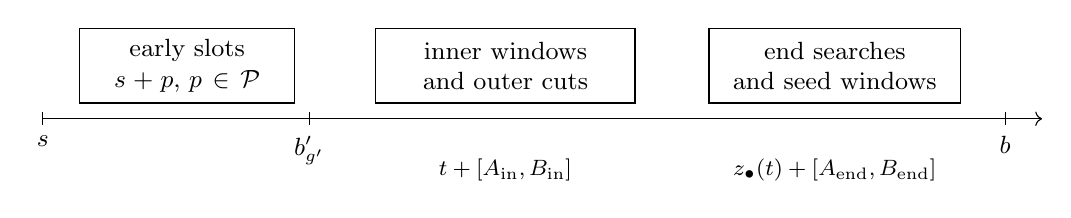
\begin{tikzpicture}[x=.94cm,y=1cm,font=\small]
 \draw[->] (0,0)--(13.5,0);
 \draw (0,-.08)--(0,.08) node[below=5pt] {$s$};
 \draw (13,-.08)--(13,.08) node[below=5pt] {$b$};
 \draw (.5,.2) rectangle (3.4,1.15);
 \node[text width=2.5cm,align=center] at (1.95,.675)
   {early slots\\$s+p$, $p\in\mathcal P$};
 \draw (4.5,.2) rectangle (8,1.15);
 \node[text width=3cm,align=center] at (6.25,.675)
   {inner windows\\and outer cuts};
 \draw (9,.2) rectangle (12.4,1.15);
 \node[text width=2.9cm,align=center] at (10.7,.675)
   {end searches\\and seed windows};
 \draw (3.6,-.08)--(3.6,.08) node[below=5pt] {$b'_{g'}$};
 \node[font=\footnotesize,align=center] at (6.25,-.65)
   {$t+[A_{\rm in},B_{\rm in}]$};
 \node[font=\footnotesize,align=center] at (10.7,-.65)
   {$z_\bullet(t)+[A_{\rm end},B_{\rm end}]$};
\end{tikzpicture}
\caption{The order of bounded data in a complete episode, schematically
and not to scale.  Both window intervals include every prescribed shifted
hypothesis.  The end anchor may be a bounded marker return or a later
first mismatch; in either case the fixed tail puts $b$ beyond all bounded
end data.}\label{schedule:schematic}
\end{figure}

\FloatBarrier

For every prefix or suffix test below, the letters needed for a check
must be present in that test's own argument and on its own reading side.
An unavailable inspection or an invalid required product interval causes
rejection; it never removes an origin from a universal check.  The
unbounded portions of the episode rule are continuation tests up to a
proposed end.  They do not require moving an unbounded inspection window
before a cut.  Lemma~\ref{schedule:inner-cuts} supplies the more precise
division of inner data between the two sides of an outer cut.

\begin{lemma}\label{episode:prefix-code}
The language $E$ is a prefix code of nonempty words.
\end{lemma}

\begin{proof}
Suppose that a complete episode is read from its beginning in a longer
word.  By Lemma~\ref{schedule:margins}, every bounded search and seed
inspection lies inside the episode, so locality gives exactly the same
search values on the longer word.  If $\eta$ is present, it gives the same
$q_0$.  If it is absent, the seed gives the same continuation, and the
already encountered first mismatch remains the first mismatch.  Thus
$q_0$, and hence $b$, cannot change.  No complete episode can be a proper
prefix of another.  Positivity follows from the strict ordering in
Lemma~\ref{schedule:margins} and from $L_{\rm tail}>1$.
\end{proof}

All these definitions commute with translation of positions.  A standalone
prefix reads from its beginning $s$ to its end $k$.  A standalone suffix
begins at $k$; an origin specified as an offset from $k$ need not itself
carry a visible letter in that suffix.  Applying the end rule at such an
origin requires the end searches and seed in the suffix and its prescribed
exact endpoint.  It does not ask the suffix to validate omitted prefix
letters.

\subsection{A guard that forces the true end}

At a proposed outer cut $k$, let the suffix test all origins
\begin{equation}\label{episode:outer-origins}
 \mathcal O_k=\{k-a:a\in\mathcal H\}.
\end{equation}
Choose once and for all a reference offset in $\mathcal H$.  The
\emph{common end guard} requires both $\eta$ and $\zeta$ to be constant
across $\mathcal O_k$, with equality of absolute positions or of the value
$\bot$.  Require all the associated bounded inspections and seed blocks.
The suffix must end exactly where the episode rule at the reference
origin prescribes, and uses the clock anchor calculated there by
\eqref{episode:clock-anchor}.

\begin{lemma}[Shared end and clock anchor]\label{episode:shared-end}
Let a word in $E^*$ have first episode beginning at $s$, sampling origin
$t=s+L$, endpoint $b$, and clock anchor $q$.  Let $k=t+a$ be any genuine
outer cut, with $a\in\mathcal H$.  If a suffix starting at $k$ satisfies
the common end guard, then its consumed endpoint is exactly $b$ and the
clock anchor it uses is exactly $q$.

Conversely, the actual suffix of that episode from $k$ to $b$ satisfies
the guard whenever both end searches at $t$ are unchanged under every
shift divisible by $B$ with absolute value at most $w$.
\end{lemma}

\begin{proof}
Because $k=t+a$ for an actual offset $a\in\mathcal H$, the set
$\mathcal O_k$ contains $t$. All its other origins differ from $t$ by
$\mathcal H-\mathcal H$. Lemma~\ref{schedule:margins} puts their
bounded end data inside the first episode and after $k$. A proposed
suffix must supply every one of these windows. If it is too short it
rejects; otherwise it reads the genuine letters in those windows, even
if its endpoint proposal is false.

Suppose first that the common value of $\eta$ is a marker. Since $t$
is among the origins, this value is the episode's own $q_0$, and the
reference end test demands $q_0+L_{\rm tail}=b$.

In the remaining case all smaller searches are absent. Let $t_*$ be the
reference origin. Its seed and the true seed start less than
$w<d_\bullet$ apart and overlap in at least
$K_\bullet-w>d_\bullet^2$ letters. Their short-period continuations are
therefore identical by Lemma~\ref{marker:periodic}. The word agrees
with that continuation on both seeds and hence on their union. If one
seed ends earlier, there is still agreement through the end of the later
seed. Consequently the first mismatch after either seed is one and the
same position. An alleged earlier mismatch contradicts that agreement
or the true first-mismatch property. An alleged later one would pass the
true first mismatch. Thus the reference exact-end test again forces $b$.
The common value of $\zeta$ now also forces $q$: it is the true bounded
return when present, and the common $q_0$ otherwise.

Conversely, every displacement from $t$ to a member of $\mathcal O_k$
is divisible by $B$ and has magnitude less than $w$. The assumed
stability makes each search constant on this set. All windows are
available in the actual suffix by the margin lemma. A common marker
return fixes the true end immediately; in the absent case the seed
argument above fixes the common first mismatch. Hence the reference
end test succeeds and supplies the true clock anchor.
\end{proof}

We can now use the clock with genuinely independent prefix and suffix
metadata.  Even if their proposed roles differ, the guard ensures that
the two clock arguments add to the true total $\varphi(q-t)$.

\section{The first split: transmitting a state with a clock}
\label{outer:section}

The schedule and end guard now permit the first split on the episode
code $E$. We will define its update before its tests, so that successful
choices cannot change which computation an episode performs. The update
is affine on $V$ and always has the original monoid action as its linear
part. Completeness of the tests is required outside an intrinsic domain
$D\subseteq E$; soundness is required for every successful pair on $E^*$.

The clock makes that soundness feasible. Equal tags let the two factors
verify a single consistent table certificate. If their tags differ, the
clock leaves only one possible ordered pair, and the affine translation
is chosen to realize its prescribed input and output. This choice is made
on the episode's actual clock graph, including episodes for which no split
will be available.

Throughout the section an episode is $[s,b)$, with $t=s+L$ and anchors
$q_0,q$ as in Section~\ref{episode:section}. The outer cut offsets form
$\mathcal H\subset B\mathbb Z$. All inspections obey the reading-side
and rejection conventions fixed there.

\subsection{The exceptional domain and a total affine update}

Define $Z(t)$ to mean that at least one of $\eta,\zeta$ is not constant
on
\[
 \{t+v:v\in B\mathbb Z,\ |v|\le w\}.
\]
For a position $Q$, let $u=(Q-t)\bmod B$, with residues represented in
$\{0,\ldots,B-1\}$.  Define $A_*(t,Q)$ to be the disjunction of the
following three conditions:
\begin{enumerate}
\item $\varphi(Q-t)\in W$;
\item for some $0\le j\le g$ and some integer $v$ with $|v|\le w_0$,
      $f_j^u(t+v)\ne f_j^u(t)$;
\item for some $0\le j\le g$, $f_j^u(t)=\bot$, but the inclusive
      interval
      $[z_j(t),z_j(t)+H_u+H_{\rm ext}]$ contains an inner marker.
\end{enumerate}
In the second condition the index $u$ is held fixed as $t$ is shifted.
The search values are absolute positions, with $\bot$ equal only to
$\bot$.  Set
\begin{equation}
 D=\{e\in E: Z(t)\ \text{or}\ A_*(t,q)\}.
 \label{outer:exceptional-domain}
\end{equation}
The episode determines both predicates without choosing a split.
Thus $D$ is a fixed language. In particular, failure of a particular
choice of tag is not its definition; the same $D$ must serve every input
state and every pair of independently chosen tags.

For $A,C\in M$, write
\begin{equation}
 f_{A,C}(a_1,\ldots,a_g)\colon
 v\longmapsto vA a_1\cdots a_g C.
 \label{outer:product-table}
\end{equation}
This is a map from $M^g$ into $\operatorname{End}_{\rm lin}(V)$.
For every such map, use the shift table $\beta_{f_{A,C}}$ fixed in
Lemma~\ref{alg:shift-table}.  We define $F_e\colon V\to V$ on
\emph{every} complete episode, including every episode in $D$:
\begin{enumerate}
\item If $\mathcal E_{\varphi(q-t)}$ is the singleton off-diagonal edge
      $\{(\alpha,\lambda)\}$, put
      \begin{equation}
      F_e(v)=vT_{s,b}+Y(\lambda)-X(\alpha)T_{s,b}.
      \label{outer:off-diagonal-update}
      \end{equation}
\item Otherwise put $u=(q-t)\bmod B$.  If at least one
      $f_j^u(t)$ is absent, put $F_e(v)=vT_{s,b}$.
\item In the remaining case let $l_j=f_j^u(t)$ for $0\le j\le g$.
      Their order is $l_0<\cdots<l_g$ by the schedule.  Set
      \[
      A=T_{s,l_0},\qquad C=T_{l_g,b},\qquad
      d_i=T_{l_{i-1},l_i}\quad(1\le i\le g).
      \]
      Then put
      \begin{equation}
      F_e(v)=v f_{A,C}(\mathbf d)+\beta_{f_{A,C}}(\mathbf d).
      \label{outer:table-update}
      \end{equation}
\end{enumerate}
These three cases define exactly one map on every episode. The first
case is unambiguous by the clock alternative. The other cases cover all
graphs contained in the diagonal, including the empty graph, with the
actual residue and actual marker data. In the third case,
$A d_1\cdots d_g C=T_{s,b}$, so all three formulas have the same
prescribed linear part. Hence $F_e$ is total and deterministic even on
$D$, and no cancellation or inverse in $M$ has entered its definition.

\subsection{The two independently chosen tags}

For each $x,y\in V$ we define languages $P_x,Q_y$ by finite unions
over tags.  A prefix factor is read on $[s,k)$, and a suffix factor
on $[k,b)$.  These positions describe the tests in their own relative
coordinates; they do not give either factor access to the other one.

Every prefix test chooses a tag $\alpha$, requires
$x=X(\alpha)$, chooses a cut of the form specified by that tag, and
requires
\begin{equation}
                 \varphi(k-t)\in I_\alpha.
 \label{outer:prefix-clock}
\end{equation}
Every suffix test chooses an independent tag $\lambda$.  It performs
the shared-end guard of Lemma~\ref{episode:shared-end}, using all
origins $k-a$, $a\in\mathcal H$.  More explicitly, both end searches
$\eta,\zeta$ must be constant over these origins; the suffix must
end exactly as prescribed at one fixed reference origin; all the
required seed and inspection data must be present.  Let $q$ denote
the clock anchor so obtained.  The suffix requires
\begin{equation}
 y=Y(\lambda),\qquad
 \varphi(q-k)\in J_\lambda,\qquad
 u(\lambda)=(q-k)\bmod B.
 \label{outer:suffix-clock}
\end{equation}
The field $u(\lambda)$ is part of the suffix's tag.  The additional
tests depend on the tag's form as follows.

\paragraph{Main tags.}
A main tag has fields $(j,u,A,C,\mathbf d_{-j},X,Y)$.
Its prefix chooses one of the cuts
\[
                 k=t+c_j+aB,\qquad 0\le a<R.
\]
Using the tag's fixed index $u$, it requires the boundary searches
$f_0^u(t),\ldots,f_{j-1}^u(t)$ to be present.  It checks $A$ and
the listed products $d_i$ for $i<j$ against the intervals on its
side of the cut.  For $a\in M$, let $\mathbf d[j\leftarrow a]$
denote the tuple formed by inserting $a$ into position $j$ of the
tag's listed entries.  The prefix also checks the finite table certificate
\begin{equation}
 X f_{A,C}(\mathbf d[j\leftarrow a])
 +\beta_{f_{A,C}}(\mathbf d[j\leftarrow a])=Y
 \qquad(a\in M).
 \label{outer:main-certificate}
\end{equation}
The fields used in this certificate are the tag's fields, not an
assumption about the unseen half of the episode.

A suffix with main tag $(j,u,A,C,\mathbf d_{-j},X,Y)$ requires all
searches with labels $j,\ldots,g$, with this fixed $u$, to be present
and to have identical absolute positions at every origin
\begin{equation}
                  k-c_j-aB,\qquad 0\le a<R.
 \label{outer:main-hypotheses}
\end{equation}
Using those common positions, it checks $d_i$ for $i>j$ and $C$
against the suffix.  Every inspection is required at every origin
in \eqref{outer:main-hypotheses}; an unavailable inspection rejects
the suffix instead of discarding that origin.  The reading-side
separation in the main-cut schedule ensures that these are suffix
tests even when the tag is not the tag chosen by a paired prefix.

\paragraph{Periodic tags.}
A periodic tag has fields $(j,u,m_p,X,Y)$, where $0\le j\le g$.
Its prefix chooses a cut
\[
 k=z_j(t)+H_u+L_{\rm lag}+aB,\qquad 0\le a<n d N_M,
\]
checks $f_j^u(t)=\bot$, and checks $m_p=T_{s,k}$.
A suffix with this tag requires
\begin{equation}
                       Y=X m_p T_{k,b},
 \label{outer:periodic-certificate}
\end{equation}
where $b$ is its own exact endpoint, as required by the shared-end
guard.  It does not presume that the independently chosen prefix
has the same tag.

These rules completely specify $P_x$ and $Q_y$.  All choices of
tags, cut offsets, table entries, and origins belong to previously
fixed finite sets.  In particular, the universal certificate in
\eqref{outer:main-certificate} is a finite Boolean test.

\subsection{Correctness for arbitrary successful pairs}

\begin{proposition}[First split]\label{outer:split}
For the total updates $F_e$ above and $D\subseteq E$ from
\eqref{outer:exceptional-domain}, the languages $P_x,Q_y$ have the
following properties.
\begin{enumerate}
\item On any word in $E^*$, a match of $P_xQ_y$ beginning at the
      beginning of the word consumes exactly its first episode $e$
      and satisfies $F_e(x)=y$.
\item For every $e\in E\setminus D$ and every $x\in V$, some cut
      of $e$ gives a match of $P_xQ_{F_e(x)}$.
\end{enumerate}
There is no match on the empty word.
\end{proposition}

\begin{proof}
\emph{Soundness.} Let independent tags $\alpha,\lambda$ witness a
successful pair at the beginning of a word in $E^*$. The prescribed
prefix length is positive and, on a nonempty such word, ends at an outer
cut strictly within its first episode. The true origin is among the
origins checked by the suffix. Lemma~\ref{episode:shared-end} therefore
forces the true endpoint $b$ and clock anchor $q$, even when the two tags
propose different forms or boundary indices. On the empty word the
positive prefix length cannot match.

The clock tests now add using actual common positions:
\[
 \varphi(q-t)=\varphi(k-t)+\varphi(q-k)\in I_\alpha+J_\lambda.
\]
If the graph is contained in the diagonal, this edge forces
$\alpha=\lambda$. Since $k-t$ is divisible by $B$, the suffix's residue
field is the true $u=(q-t)\bmod B$. For a main tag, the actual origin
occurs among its role-specific hypotheses
\eqref{outer:main-hypotheses}. The prefix verifies boundaries through
$j-1$, the suffix verifies those from $j$ onward, and together they
verify $A,C$ and every listed interval product. All actual boundaries
are therefore present. Substituting the actual missing product into the
universal certificate \eqref{outer:main-certificate} gives
$F_e(x)=y$ under \eqref{outer:table-update}.

For an equal periodic tag, the prefix establishes absence of the actual
search with the true index $u$. The linear case of $F_e$ therefore
applies. Its verified $m_p=T_{s,k}$ and the suffix certificate imply
\[
 y=xm_pT_{k,b}=xT_{s,b}=F_e(x).
\]
An empty clock graph cannot produce either successful case.

If the graph instead consists of one off-diagonal edge, the successful
pair must be exactly that edge. The separate state checks say
$x=X(\alpha)$ and $y=Y(\lambda)$. Formula
\eqref{outer:off-diagonal-update} was defined to give this equality
$F_e(x)=y$. No agreement of their other fields is needed. This exhausts
all successful pairs and proves soundness.

\emph{Completeness.} Fix $e\in E\setminus D$ and an arbitrary input
$x\in V$. The negation of $Z(t)$ supplies the common end guard at every
scheduled outer cut. Put $u=(q-t)\bmod B$. Since
$\varphi(q-t)\notin W$, every tag $\alpha$ has a ball of radius $\rho$
in $I_\alpha\cap(\varphi(q-t)-J_\alpha)$, and the clock graph is the
full diagonal. We must find a cut that hits the ball for a tag whose
letter tests and certificate are correct.

If all searches $f_i^u(t)$ are present, take their true products
$A,C,\mathbf d$. The shift-table lemma supplies a coordinate $j$ that
can be omitted for this tuple and input. Give the main tag those true
fields and $X=x$, $Y=F_e(x)$. Its universal certificate then holds. The
clock values at its main cuts are
\[
 \varphi(c_j)+\varphi(aB),\qquad 0\le a<R,
\]
a translate of the fixed net, so one cut meets its ball. At that cut,
every alternative role-specific origin is $t+(a-a')B$ with displacement
of magnitude less than $w_0$. The stability part of $\neg A_*(t,q)$,
with $u$ fixed, makes the required future marker positions agree.
The remaining tests are actual products on the proper reading sides.
Thus the main pair succeeds.

If some $f_j^u(t)$ is absent, write $z=z_j(t)$. The last part of
$\neg A_*(t,q)$ makes $[z,z+H_u+H_{\rm ext}]$ markerless.
Lemma~\ref{schedule:periodic-cuts} gives a period $d'<d$ and cuts
\begin{equation}
 k_a=k_0+a d'N_MB,\qquad 0\le a<n,\qquad
 k_0=z+H_u+L_{\rm lag},
 \label{outer:periodic-progression}
\end{equation}
whose prefix products share one value $m_p$. Choose the periodic tag
with these $j,u,m_p$ and with $X=x$, $Y=xT_{s,b}=F_e(x)$.
It is a single tag for the whole progression: constancy of $m_p$ follows
from eventual periodicity of monoid powers, without cancelling an earlier
factor. The same lemma shows that its clock values traverse a translate
of the full clock image, and hence include a translate of the fixed net.
One therefore hits the ball for this tag. The marker-absence inspections
are before the cut by the lag condition, and the suffix certificate
$Y=Xm_pT_{k_a,b}$ follows from $m_pT_{k_a,b}=T_{s,b}$. The common end guard already holds. This proves
completeness in the periodic case as well, for every input $x$.
\end{proof}

We now have the first split interface on all of $E$, with the same
updates $F_e$ reserved for its skipped episodes. To complete the sequence
computation, it remains to handle $D^*$. The defining exceptional
predicate, which was an obstruction to the clock construction, will
serve as a witness to the origin at an earlier stencil cut. The next
section proves that this witness is usually unique across the entire
stencil.

\section{Recovering the cut on exceptional episodes}
\label{decode:section}

Every episode in $D$ satisfies $Z(t)\lor A_*(t,q)$. This is useful
information for a suffix: if its prefix ended at $k=s+p$, the true origin
is one of the finitely many candidates $k+L-p'$, $p'\in\mathcal P$.
We will use the exceptional predicate to identify it.

Two issues must be resolved separately. First, false candidate origins
must be sparse over \emph{all} stencil slots, not just those whose
metadata might be correct. Second, a suffix proposing an incorrect end
must not make the true witness disappear. We first count using actual
episode data. We then give a suffix test that obtains precisely enough
of those data before it asks for uniqueness, and checks the decoded
origin's end afterward.

\subsection{A bounded list of possible clock anchors}

Fix a complete episode $[s,b)$ and its actual origin $t=s+L$.
For every pair $p,p'\in\mathcal P$, set
\[
       \delta=p-p',\qquad \tau=t+\delta.
\]
The distinct-slot differences are distinct as integers and modulo
$B$, are separated from one another by more than $2w_0+2$, and
satisfy $|\delta|\le h$.  The identical-slot pairs all give $t$.
Evaluate the bounded larger end search $\zeta(\tau)$ on the
actual episode.

If one of these larger searches is absent, then every smaller
search $\eta(\tau)$ in this collection is absent.  Indeed, a
marker eligible for a smaller search at any one origin has
distance at most $\max_u D^0_u+2h$ from the end-search center at
any other origin.  The inequality
\begin{equation}
                 \max_u D^0_u+2h<\min_u D^1_u
 \label{decode:two-searches}
\end{equation}
makes it eligible for that larger search, whatever residue index
it has at the latter origin.  This would contradict the absent
larger search.

In this absence case the seeds at all these origins have short
periods.  Their starting positions differ by at most $2h$; the
seed length and marker separation ensure an overlap of at least
$d_\bullet^2$.  Lemma~\ref{marker:periodic} gives the same
two-sided periodic continuation for all seeds.  They agree with
the episode on their union, so their first subsequent mismatch
is the same position $q_0$.  This is the actual episode's mismatch
anchor, because its own smaller search is absent.  Define
\begin{equation}
 Q_\tau=
 \begin{cases}
  \zeta(\tau),&\zeta(\tau)\ne\bot,\\
  q_0,&\zeta(\tau)=\bot.
 \end{cases}
 \label{decode:anchors}
\end{equation}
The second case is used only when a larger search is absent,
so the preceding argument always supplies its $q_0$.
In particular $Q_t=q$.

\begin{lemma}[Number of possible anchors]\label{decode:anchor-list}
For a fixed actual episode, the values $Q_\tau$ in
\eqref{decode:anchors}, over all $p,p'\in\mathcal P$, belong to a
set $\mathcal Q$ of at most $20$ positions.
\end{lemma}

\begin{proof}
Every present $\zeta(\tau)$ is an end marker in
\[
 [z_\bullet(t)-h-\max_uD^1_u,
   z_\bullet(t)+h+\max_uD^1_u].
\]
Since $\max_uD^1_u=3d_\bullet+(B-1)S_\bullet$ and
$d_\bullet>10BS_\bullet+10(h+w+1)$, this interval has length
strictly less than $(31/5)d_\bullet$.  End markers have separation
at least $d_\bullet$, so it contains at most seven of them.
There is at most one additional value, the shared mismatch $q_0$.
In particular the asserted bound of $20$ holds.
\end{proof}

\subsection{Counting every false origin in the stencil}

We now count the ordered pairs with $p\ne p'$ for which the
translated origin satisfies the exceptional predicate.  All
marker decisions can be made in one common two-sided extension:
the margin construction makes every inspection used below
internal to the episode, including the shifted searches.

\begin{proposition}[Whole-stencil sparsity]\label{decode:sparsity}
For each complete episode and the positions $Q_\tau$ in
\eqref{decode:anchors},
\begin{equation}
 \#\bigl\{(p,p')\in\mathcal P^2:p\ne p',\
 Z(t+p-p')\ \text{or}\
 A_*(t+p-p',Q_{t+p-p'})\bigr\}<\mu.
 \label{decode:whole-stencil-bound}
\end{equation}
This bound includes every ordered distinct-slot pair, independently
of the kinds assigned to its slots.
\end{proposition}

\begin{proof}
We separately count end-search instability, and the three causes
in $A_*$.  Write $\delta=p-p'$ and $\tau=t+\delta$.

\paragraph{End-search instability costs at most four pairs.}
If an end search changes when $\tau$ is replaced by $\tau+v$,
where $v\in B\mathbb Z$ and $|v|\le w$, the eligibility of some
marker changes.  Otherwise the set of eligible markers, and
hence its leftmost member or its absence, would be unchanged.
For that marker $m_e$, the index
\[
                 u=(m_e-z_\bullet(t)-\delta)\bmod B
\]
is unchanged during this shift, since $v$ is divisible by $B$.
Thus for some $\sigma\in\{0,1\}$ and one of the two signs,
\begin{equation}
 \bigl|m_e-(z_\bullet(t)+\delta\mathbin{\pm}D^\sigma_u)\bigr|
 \le w.
 \label{decode:end-crossing}
\end{equation}
Fix the search $\sigma$ and the sign.  As $\delta$ varies in
$[-h,h]$ and $u$ varies in $\{0,\ldots,B-1\}$, all possible
markers in \eqref{decode:end-crossing} lie in an interval of
diameter at most
\[
                 2h+(B-1)S_\bullet+2w<d_\bullet.
\]
There is at most one end marker in that interval.  For this fixed
marker the indices $u$ are distinct for the distinct-slot
differences, because those differences are distinct modulo $B$.
Two target positions in \eqref{decode:end-crossing} are then
separated by at least $S_\bullet-2h>2w$.
At most one pair can satisfy \eqref{decode:end-crossing} for this
search and sign.  The two searches and two signs therefore
contribute at most four pairs in total.

\paragraph{Fixing an anchor makes the clock count uniform.}
For each fixed $Q\in\mathcal Q$, the clock part of $A_*(\tau,Q)$
is
\[
 \varphi(Q-t)+\varphi(p')-\varphi(p)\in W.
\]
Apply Lemma~\ref{clock:robust} at the translate
$\varphi(Q-t)$, with the realized roster values $\varphi(p)$.
It counts at most $c_{\rm cl}\log(2m)$ ordered distinct-slot
pairs.  Its uniformity in the translate permits this application
for every actual value of $Q$, including an unbounded mismatch
position.  There are only $|\mathcal Q|\le20$ such applications.

\paragraph{For each fixed anchor and label, inner-marker failures
cost at most three pairs.}
Fix $Q\in\mathcal Q$ and $j\in\{0,\ldots,g\}$.
For each $\delta$ write
\[
 z=z_j(t)+\delta,\qquad u=(Q-t-\delta)\bmod B.
\]
In the stability part of $A_*$, the index $u$ is held fixed while
$z$ is shifted by an integer of magnitude at most $w_0$.
The union of all these possible left-endpoint positions has
diameter $2h+2w_0<d$, so it contains at most one inner marker.
The distinct differences $\delta$ are separated by more than
$2w_0+2$.  Consequently at most one pair has its left endpoint
within $w_0$ of this marker.  Charge that pair, if present, to
the left endpoint.

For any remaining pair, no marker crosses the left endpoint
during the allowed shifts.  The first marker on or after $z$,
if it exists, is therefore fixed during those shifts.
A change of the first-marker search can now occur only if this
marker is within $w_0$ of the right endpoint $z+H_u$.
Also, if the search on $[z,z+H_u]$ is absent but the extended
interval contains a marker, its first marker lies in
$(z+H_u,z+H_u+H_{\rm ext}]$.
Thus either remaining failure puts the first marker on or after
$z$ within $\max(H_{\rm ext},w_0)$ of $z+H_u$.

As $z$ ranges over its sweep of diameter $2h<d$, at most two
positions can play this first-marker role: a marker within the
sweep, and the first marker after the sweep.  If no such marker
exists, there is no pair to charge to it.
For distinct-slot differences the indices
$u=(Q-t-\delta)\bmod B$ are all distinct.  The spacing of the
widths in the schedule gives, for different such differences,
\begin{align*}
 |(z_j(t)+\delta+H_u)-(z_j(t)+\delta'+H_{u'})|
 &\ge |H_u-H_{u'}|-|\delta-\delta'|\\
 &>2\max(H_{\rm ext},w_0)+2.
\end{align*}
Each of the two possible first markers can therefore account for
at most one pair.  Together with the possible left-endpoint pair,
this is at most three pairs for fixed $Q,j$.

Combining the counts, the left side of
\eqref{decode:whole-stencil-bound} is at most
\begin{equation}
 4+20\bigl(c_{\rm cl}\log(2m)+3(g+1)\bigr)
 <20\bigl(c_{\rm cl}\log(2m)+4(g+1)\bigr)+10<\mu.
 \label{decode:budget}
\end{equation}
The last inequality is precisely the multiplicity choice in
the schedule.  Counting all pairs for each fixed $Q$, rather
than only pairs assigned that $Q$, is an upper bound and makes
the use of the clock and width estimates uniform.  Taking the
union over the short list $\mathcal Q$ completes the proof.
\end{proof}

There are two levels to this estimate. At a \emph{fixed} anchor $Q$,
distinct displacement residues give distinct width indices, so right-end
failures are sparse. The anchor list then permits at most twenty such
counts. The estimate includes all ordered pairs; no knowledge of the
correct kind was used to obtain it. We can now turn it into a decoder
without assuming that a suffix's proposed endpoint is correct.

\subsection{A decoder that also verifies its endpoint}

We next give an actual test on a suffix beginning at $k$.
For each slot $p'\in\mathcal P$ form the candidate origin
\begin{equation}
                        \tau_{p'}=k+L-p'.
 \label{decode:candidate-origins}
\end{equation}
These are positions relative to the suffix; the origin itself
need not be a visible letter.  All of the following inspections,
including every shifted search needed to evaluate $Z$ and $A_*$,
are mandatory.  If a required window is absent from the suffix,
the test rejects.

First compute every $\zeta(\tau_{p'})$.  If at least one is
absent, require all $\eta(\tau_{p'})$ to be absent, read every
candidate seed, and require the suffix to end exactly according
to the end rule at one fixed reference candidate.  This includes
agreement with that reference seed's periodic continuation up
to its first subsequent mismatch, and exactly $L_{\rm tail}$
letters from that mismatch to the proposed endpoint.  Denote
its verified mismatch position by $q_{\rm ref}$.  For candidate
origins with absent $\zeta$, use $Q_{\tau_{p'}}=q_{\rm ref}$.
For every candidate with present $\zeta$, always use
$Q_{\tau_{p'}}=\zeta(\tau_{p'})$.
If all the larger searches are present, no reference mismatch
test is needed at this step; all these $Q$'s are bounded search
returns.

Now require that exactly one slot $p'$ satisfy
\begin{equation}
         Z(\tau_{p'})\ \text{or}\
         A_*(\tau_{p'},Q_{\tau_{p'}}).
 \label{decode:unique-witness}
\end{equation}
This is uniqueness over all slots, without any restriction to
particular kinds or guessed table values.  Finally, after
decoding this slot, require exact consumption according to the
end rule at its candidate origin in \emph{all} cases, including
the case where all larger searches were present.

Figure~\ref{decode:two-guards-figure} separates the two anchor roles and
records the order of these end checks. The reference guard belongs only
to the branch with an absent larger search. The decoded origin's exact
end is checked in both branches.
\begin{figure}[htbp]
\centering
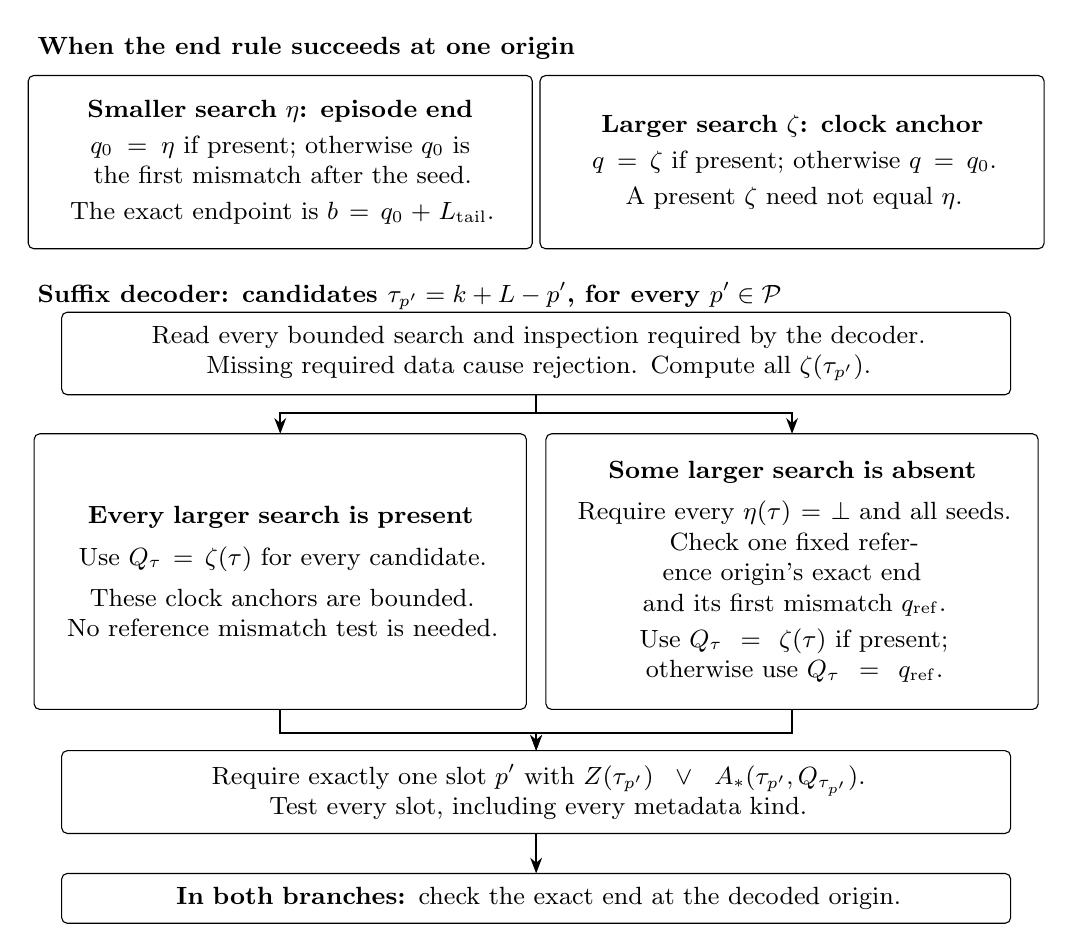
\begin{tikzpicture}[
  font=\small,
  box/.style={draw,rounded corners=2pt,align=center,inner sep=5pt},
  flow/.style={-{Stealth[length=2mm]},semithick},
  every node/.style={outer sep=0pt}
]
\node[anchor=west,font=\small\bfseries] at (-6.45,0)
  {When the end rule succeeds at one origin};
\node[box,text width=6.05cm,minimum height=2.2cm] (endrole)
  at (-3.25,-1.45)
  {\textbf{Smaller search $\eta$: episode end}\\[2pt]
   $q_0=\eta$ if present; otherwise $q_0$ is\\
   the first mismatch after the seed.\\[2pt]
   The exact endpoint is $b=q_0+L_{\rm tail}$.};
\node[box,text width=6.05cm,minimum height=2.2cm] (clockrole)
  at (3.25,-1.45)
  {\textbf{Larger search $\zeta$: clock anchor}\\[2pt]
   $q=\zeta$ if present; otherwise $q=q_0$.\\[2pt]
   A present $\zeta$ need not equal $\eta$.};
\begin{scope}[yshift=-3mm]
\node[anchor=west,font=\small\bfseries] at (-6.45,-2.85)
  {Suffix decoder: candidates $\tau_{p'}=k+L-p'$, for every $p'\in\mathcal P$};
\node[box,text width=11.7cm] (read) at (0,-3.58)
  {Read every bounded search and inspection required by the decoder.\\
   Missing required data cause rejection. Compute all $\zeta(\tau_{p'})$.};
\node[box,text width=5.9cm,minimum height=3.5cm] (present)
  at (-3.25,-6.35)
  {\textbf{Every larger search is present}\\[4pt]
   Use $Q_\tau=\zeta(\tau)$ for every candidate.\\[4pt]
   These clock anchors are bounded.\\
   No reference mismatch test is needed.};
\node[box,text width=5.9cm,minimum height=3.5cm] (absent)
  at (3.25,-6.35)
  {\textbf{Some larger search is absent}\\[4pt]
   Require every $\eta(\tau)=\bot$ and all seeds.\\
   Check one fixed reference origin's exact end\\
   and its first mismatch $q_{\rm ref}$.\\[2pt]
   Use $Q_\tau=\zeta(\tau)$ if present;\\
   otherwise use $Q_\tau=q_{\rm ref}$.};
\draw[flow] (read.south) -- ++(0,-.23) -| (present.north);
\draw[flow] (read.south) -- ++(0,-.23) -| (absent.north);
\node[box,text width=11.7cm] (unique) at (0,-9.15)
  {Require exactly one slot $p'$ with
   $Z(\tau_{p'})\ \lor\ A_*(\tau_{p'},Q_{\tau_{p'}})$.\\
   Test every slot, including every metadata kind.};
\draw[flow] (present.south) -- ++(0,-.3) -| (unique.north);
\draw[flow] (absent.south) -- ++(0,-.3) -| (unique.north);
\node[box,text width=11.7cm] (finish) at (0,-10.5)
  {\textbf{In both branches:} check the exact end at the decoded origin.};
\draw[flow] (unique.south) -- (finish.north);
\end{scope}
\end{tikzpicture}
\caption{The two end searches and the suffix decoder. At a genuine stencil
 cut, absence of one larger search forces all smaller searches to be absent.
 The overlapping seeds then have a common first mismatch, verified by the
 reference end check in the right branch. In the left branch, every clock
 anchor is bounded data, even if the episode end comes from a later mismatch.
 Both branches test uniqueness over the entire stencil and then check the
 exact end at the decoded origin.}
\label{decode:two-guards-figure}
\end{figure}

\FloatBarrier

\begin{lemma}[Suffix decoder]\label{decode:decoder}
Suppose the suffix test just described is paired with a genuine
stencil prefix $[s,k)$, $k=s+p$, of a first episode $e\in D$ in a
word of $D^*$.
If the suffix test succeeds, it decodes the actual slot $p$ and
consumes exactly to the actual endpoint $b$.
Conversely, on the actual suffixes of a fixed episode $e\in D$,
fewer than $\mu$ actual slots fail the decoder.  In particular,
each kind has a copy at which decoding succeeds.
\end{lemma}

\begin{proof}
\emph{The true witness survives before uniqueness.} Pair the suffix
with a genuine prefix cut $k=s+p$. Its candidates are exactly
$t+p-p'$, including $t$ at $p'=p$. Every bounded inspection for these
candidates lies inside the true first episode by the margin lemma, and
is mandatory in the proposed suffix. Thus a suffix that reaches the
uniqueness test has read the genuine values of all those inspections,
regardless of whether its proposed end is too early or too late.

If one larger search is absent, the decoder requires absence of all
smaller searches and reads every seed. The true seed is among them.
The overlap argument used above makes their periodic continuations the
same, with agreement throughout their union. Consequently the reference
exact-end check identifies the true first mismatch $q_0$: an earlier
claimed mismatch contradicts agreement before $q_0$, and a later one
would fail to detect $q_0$. The reference guard therefore forces the true
end in this branch. All tested anchors agree with
\eqref{decode:anchors}, so at $t$ the exceptional predicate is true.

If instead all larger searches are present, every candidate anchor is a
bounded return, already read inside the true episode. In particular the
true candidate uses $Q_t=\zeta(t)=q$. No assumption about the proposed
end has been made or is needed to evaluate its predicate. Because the
first episode belongs to $D$, the true candidate again satisfies
\eqref{decode:unique-witness}. Notice that this branch need not have a
bounded episode end: the true smaller search can still be absent.

\emph{Uniqueness and endpoint soundness.} In either branch the actual
slot is a witness before uniqueness is imposed. Hence a successful
uniqueness test must choose that slot $p$. The final end check is now the
end rule at the true origin and forces the actual endpoint $b$. This
last check is imposed in both branches. It cannot be omitted merely
because all larger searches are present.

\emph{Completeness at almost every slot.} Use the actual suffix for each
slot of a fixed $e\in D$. The margin lemma supplies every required
window. When one larger search is absent, implication
\eqref{decode:two-searches} makes all smaller searches absent and the
common-seed argument makes the reference guard pass. For each actual slot
$p$, the computed anchors are the restriction of \eqref{decode:anchors}
to its candidates $t+p-p'$: a present $\zeta$ supplies its return,
while an absent $\zeta$ uses the common actual mismatch $q_0$.
Thus the true witness and its final end check pass. Only an additional
witness can prevent success.

For each unsuccessful actual slot $p$, select one additional witnessing
slot $p'\ne p$. Then $(p,p')$ is counted by
\eqref{decode:whole-stencil-bound}. Different unsuccessful actual slots
have different first coordinates, so this selection is injective.
Fewer than $\mu$ slots therefore fail. Since every kind has $\mu$
copies, at least one copy of each kind succeeds.
\end{proof}

The two end-search sizes are essential to this test.  If a false
origin has absent larger search, all the smaller searches,
including the true one, are absent and the shared mismatch is
already the actual endpoint anchor.  Otherwise every candidate
clock anchor is bounded data.  Thus the decoder never needs to
look for an unverified future mismatch beyond a short true
episode merely to decide a false origin's witness.

\section{The second split: transmitting a table through the stencil}
\label{inner:section}

At a successful early cut, the suffix can now recover the actual stencil
slot and hence its metadata. That removes the problem of independently
chosen kinds, but an interval crossing the cut is still unreadable. We
handle it using the arbitrary-function form of the shift-table lemma.

The suffix first describes the later computation by a table indexed by
the monoid product of the entire early region. The table has an entry for
every monoid value, not just values realized by prefixes. Composing this
table with the product of the early block values yields a total
function of the tuple. The shift-table lemma supplies a deterministic
affine correction for that function, and one block can then be omitted
for each input state.

\subsection{A total table computed from later letters}

Write $b'_*=b'_{g'}$, the last fixed stencil boundary, and let
$e=[s,b)\in D$.  The homogeneous lift of $F_e$ is the linear map
$\widehat F_e\colon U\to U$, where $U=V\oplus\mathbf F_2$.
If $F_e(v)=vL_e+\gamma_e$, then
\begin{equation}
              \widehat F_e(v,c)=(vL_e+c\gamma_e,c).
 \label{inner:homogeneous-update}
\end{equation}
All marker searches, outer boundaries, and end data occur after
$b'_*$ by Lemma~\ref{schedule:margins}.  Hence the suffix of the
episode starting at $b'_*$, together with its origin and anchors,
determines the following table for every $m'\in M$.

Set $D_b=T_{b'_*,b}$ and $m_b(m')=m'D_b$.  Define an affine map
$H_{e,m'}\colon V\to V$ by the same three cases as $F_e$:
\begin{enumerate}
\item If the actual clock graph is the singleton off-diagonal
      edge $\{(\alpha,\lambda)\}$, put
      \[
      H_{e,m'}(v)=v m_b(m')+Y(\lambda)-X(\alpha)m_b(m').
      \]
\item Otherwise use $u=(q-t)\bmod B$.  If at least one actual
      $f_j^u(t)$ is absent, put $H_{e,m'}(v)=v m_b(m')$.
\item In the remaining case all these searches are present; write their values as
      $l_0<\cdots<l_g$, and put
      \[
      A(m')=m'T_{b'_*,l_0},\qquad C=T_{l_g,b},\qquad
      d_i=T_{l_{i-1},l_i}.
      \]
      With $f_{A(m'),C}$ from \eqref{outer:product-table}, put
      \[
      H_{e,m'}(v)=
      v f_{A(m'),C}(\mathbf d)
      +\beta_{f_{A(m'),C}}(\mathbf d).
      \]
\end{enumerate}
Define
\begin{equation}
 \psi_e\colon M\longrightarrow\operatorname{End}_{\rm lin}(U),
 \qquad \psi_e(m')=\widehat H_{e,m'}.
 \label{inner:total-table}
\end{equation}
The hat denotes the homogeneous lift in
\eqref{inner:homogeneous-update}. For every $m'$, including an impossible
prefix product, associativity in the third case gives
\[
 A(m')d_1\cdots d_g C
   =m'T_{b'_*,l_0}T_{l_0,l_g}T_{l_g,b}
   =m'T_{b'_*,b}=m_b(m').
\]
Thus the affine formula and its linear lift are defined for every entry.
Only after the table has been defined do we substitute the actual early
product, obtaining
\begin{equation}
                    \psi_e(T_{s,b'_*})=\widehat F_e.
 \label{inner:actual-table-entry}
\end{equation}

Every letter-dependent quantity here is read after $b'_*$: marker
positions, anchor data, inter-boundary products, and products from
$b'_*$ to later positions. The hypothetical value $m'$ is simply a
finite algebraic input. The calculation does not search for omitted
prefix letters, and it does not query graph languages for sequences of
episodes.

Apply exactly the same formulas under a proposed suffix origin once its
end rule and all necessary data are available. If a required interval is
missing or its endpoints are in the wrong order, reject the entire suffix
test. Do not discard that origin, and do not discard individual values of
$m'$ from the table. This separates the availability of actual suffix
letters from the total algebraic domain of $\psi_e$. At the true origin
all required intervals are available by the margin lemma.

\subsection{The affine update on the exceptional domain}

For $1\le i\le g'$ put
\[
                         d'_i=T_{b'_{i-1},b'_i}.
\]
For any table $\psi\colon M\to\operatorname{End}_{\rm lin}(U)$,
define
\begin{equation}
 f'_\psi(a_1,\ldots,a_{g'})=\psi(a_1\cdots a_{g'}).
 \label{inner:product-table}
\end{equation}
Use the fixed shift table $\beta_{f'_\psi}$ supplied by
Lemma~\ref{alg:shift-table} with state space $U$ and dimension
$g'$.  On every $e\in D$ define
\begin{equation}
 G_e(x)=x f'_{\psi_e}(\mathbf d')+
                       \beta_{f'_{\psi_e}}(\mathbf d'),
 \qquad x\in U.
 \label{inner:affine-update}
\end{equation}
This is a deterministic total affine map on $U$.  Its linear
part is $\widehat F_e$, because
$d'_1\cdots d'_{g'}=T_{s,b'_*}$ and
\eqref{inner:actual-table-entry} applies.

The kinds in the stencil were chosen to contain all tuples
\[
          (j,x,y,\mathbf d'_{-j},\psi),
\]
where $1\le j\le g'$, $x,y\in U$,
$\mathbf d'_{-j}\in M^{g'-1}$, and
$\psi\colon M\to\operatorname{End}_{\rm lin}(U)$ is arbitrary.
The $\mu$ copies of a kind have distinct cut offsets but the same
fields.  A cut of block $j$ lies strictly inside
$(b'_{j-1},b'_j)$, so all listed block products except the omitted
$j$th product can be checked on one side or the other.

For $x,y\in U$ define inner prefix and suffix languages
$\widetilde P_x,\widetilde Q_y$ as follows.
A prefix chooses a slot $p\in\mathcal P$ and has exactly length
$p$, so its endpoint is $k=s+p$.  If the slot's kind is
$(j,x_p,y_p,\mathbf a_{-j},\psi)$, it requires $x_p=x$ and
checks all listed earlier block products $a_i=d'_i$ for $i<j$.
For $a\in M$, write $\mathbf a[j\leftarrow a]$ for the tuple
formed by inserting $a$ into the listed entries at position $j$.
The prefix also checks the finite certificate
\begin{equation}
 x_p f'_\psi(\mathbf a[j\leftarrow a])
 +\beta_{f'_\psi}(\mathbf a[j\leftarrow a])
 =y_p\qquad(a\in M).
 \label{inner:certificate}
\end{equation}
The prefix does not try to check the later entries or the table
$\psi$ against letters it cannot see.

A suffix beginning at $k$ performs the complete decoder of
Lemma~\ref{decode:decoder}, including its reference end guard
when called for and its final decoded-origin end guard.
Let $p$ be its decoded slot and use its kind
$(j,x_p,y_p,\mathbf a_{-j},\psi)$.  At the decoded origin the
suffix computes the actual searches, anchors, and all entries
of \eqref{inner:total-table}.  It requires that resulting table
equal the slot's $\psi$, checks $a_i=d'_i$ for $i>j$, and requires
$y_p=y$.  The comparison of tables is equality on every input
$m'\in M$.  Each required interval starts on or after the
suffix's beginning: in particular, the displacement of $b'_*$
from $k$ is the fixed positive offset $(b'_*-s)-p$, since every
stencil slot precedes the last stencil boundary.  The margin lemma
places all the data for the table after that boundary.

\begin{proposition}[Second split]\label{inner:split}
For the updates $G_e$ on $D$, the languages
$\widetilde P_x,\widetilde Q_y$ satisfy:
\begin{enumerate}
\item on a word in $D^*$, every match of
      $\widetilde P_x\widetilde Q_y$ from its beginning consumes
      exactly the first episode $e$ and has $G_e(x)=y$;
\item every $e\in D$ admits such a split for every input $x\in U$.
\end{enumerate}
Thus this split has empty skip domain.
\end{proposition}

\begin{proof}
For soundness, let an arbitrary successful pair begin a word of $D^*$.
The prefix selects a scheduled stencil length, so its endpoint $k=s+p$
lies inside the first episode. The decoder lemma forces the suffix to
select that very slot and to end at the actual episode endpoint. Thus
both factors use one kind, although this was not assumed when defining
their languages.

The prefix verifies every listed early block product, and the suffix
verifies every listed later one. It also compares its computed table
with the kind's table on \emph{all} $m'\in M$. Hence the listed products
are the actual $d'_i$ for $i\ne j$, and the table is $\psi_e$.
The actual product $d'_j$ of the interval crossing the cut is a member
of $M$, so it is covered by the universal certificate
\eqref{inner:certificate}. Substituting it proves $G_e(x)=y$.
The positive stencil length rules out a pair on the empty word.

For completeness, fix an episode $e\in D$ and any input $x\in U$.
Apply Lemma~\ref{alg:shift-table} to the total function
$f'_{\psi_e}$ at its actual tuple $\mathbf d'$. A coordinate $j$
exists on which the shifted output is constant, equal to $G_e(x)$.
Take the kind with that coordinate, the actual other products, the entire
actual table $\psi_e$, and input and output fields $x,G_e(x)$. It belongs
to the roster because all total tables were included when kinds were
chosen. Its finite certificate holds for every possible missing value.
The decoder lemma leaves at least one usable copy of this kind. At that
copy all product checks concern actual readable intervals, its table
comparison is exact, and its end checks pass. The split therefore exists
for the chosen $x$. Repeating this reasoning for each input proves the
all-input claim; neither the omitted coordinate nor the chosen copy is
required to be the same for different inputs.
\end{proof}

We have now obtained both split constructions with their full
all-input guarantees.  The inner updates $G_e$ have linear
parts $\widehat F_e$, and the outer updates $F_e$ have linear
parts equal to the original monoid action.  The remaining task
is to express each domain and each individual prefix or suffix
test with the claimed height over the original alphabet, and
then apply affine recovery and the split identity in this
order.

\section{Expressions over the original alphabet}
\label{sec:compilation}

Both split interfaces have been proved, including their universal
soundness under independent guesses. We have not yet assigned a height
to any of their component languages. Finite-state decidability of a test
would establish regularity, but would not give the height-one expressions
that the split identity needs.

The relevant restriction comes from each component's own end rule. A
marker return gives a bounded end. Otherwise a fixed periodic seed is
continued until its first mismatch, followed by a bounded tail. Hence
there is only one unbounded repeated word, and finitely many choices of
its fixed surrounding words. We first give the exact compilation lemma
for that situation, including additional end comparisons made at false
origins. This develops the template method of
\cite[Lemma~8.1 and Proposition~8.2]{HeightThirteen} and
\cite[Lemma~7.1 and Proposition~7.2]{HeightFour} for the present guards.

\subsection{Periodic templates and exact-end checks}

\begin{lemma}[Compilation on periodic templates]\label{compile:templates}
Fix a finite alphabet $\Sigma$, a finite monoid $M$, and a morphism
$T:\Sigma^*\to M$. Consider finitely many templates
\begin{equation}\label{compile:eq-template}
                     a c^i b,\qquad i\ge0,
\end{equation}
where $a,b,c\in\Sigma^*$ are fixed for each template and $c\ne\eps$.
On each template suppose acceptance is determined by a fixed finite
calculation using the following data:
\begin{enumerate}
\item letters in finitely many bounded windows at fixed integer offsets
from the argument's beginning or end;
\item order and availability of positions selected from fixed finite sets
of such offsets, with unavailable required data causing rejection;
\item monoid products on available ordered intervals between these positions,
and lengths or differences modulo fixed positive integers;
\item agreement of an interval between these positions with one of finitely
many fixed periodic continuations, together with any required mismatch
letter at its endpoint.
\end{enumerate}
Finite choices, universal tests, and uniqueness tests on fixed finite lists
are allowed in the calculation. Then the accepted words have a generalized
expression of height at most one over $\Sigma$. The same conclusion holds
after adding finitely many exceptional words.
\end{lemma}

\begin{proof}
Fix a template $ac^ib$. For sufficiently large $i$, the relative order
and availability of every pair of bounded-offset positions is fixed.
Adding another full copy of $c$ then leaves a bounded window near either
end unchanged. Products between endpoints near the same end are likewise
constant. Every interval product crossing the growing middle has form
\[
                       u\,T(c)^{i-i_0}\,v
\]
for fixed $u,v\in M$ and an integer $i_0$, after taking sufficiently
large $i$. Powers in a finite monoid are ultimately periodic. Thus all
these products, and all fixed-modulus length data, are ultimately
periodic functions of $i$.

For a comparison with a periodic continuation of period $d_0$, separate
the finitely many classes of $i$ modulo $d_0$. On a class, the phase of
every bounded endpoint is fixed. Comparisons in bounded pieces therefore
stabilize. A growing middle compares the repetition of $c$ with the
specified continuation in a fixed phase. If they disagree, a disagreement
occurs within $|c|d_0$ consecutive positions: this integer is a common
period of the two two-sided repetitions. Every sufficiently long middle
then fails the comparison. If there is no disagreement in such a block,
the entire growing comparison agrees, and only the fixed beginning and
end comparisons remain. A prescribed first mismatch is exactly an
agreement test up to a specified endpoint and a differing letter there,
so it is covered too. Bounded comparison intervals reduce to the earlier
window case.

There are only finitely many data and phase cases. Choose a threshold
and a common period beyond which their whole array is periodic. Any
fixed calculation on that finite array, including a universal check or
an exactly-one condition, has an ultimately periodic set of accepted
exponents. Such a set is a finite set together with finitely many
progressions $i_1+\ell\mathbb N$, $\ell>0$. A progression is expressed by
\[
                       ac^{i_1}(c^\ell)^*b.
\]
All its fixed powers are words over $\Sigma$, so this has height one.
A finite exceptional set contributes finitely many words. Taking finite
unions over the progressions and templates proves the assertion on the
original alphabet.
\end{proof}

An exact end check at a fixed candidate origin provides precisely the
template cover required by this lemma. If the smaller end search $\eta$
returns a marker, that marker has a bounded offset and the end is bounded.
Otherwise its seed is a fixed-length word at a fixed position, with a
short-period continuation. Let $a$ be the bounded word from the argument's
own beginning to the seed's right endpoint. Make finite choices of $a$,
the continuation's period and phase, and the tail of length
$L_{\rm tail}$ starting at the first mismatch. If the mismatch follows
$i$ full copies of the period word and one partial copy, put the fixed
partial copy and tail into $b$ in \eqref{compile:eq-template}. Require the
first letter of the tail to differ from the periodic continuation. These
choices give a finite template cover, with bounded cases handled separately.

This is a statement about the suffix language itself. Its proposed origin
is one of finitely many offsets from its own beginning, and its own end
check yields the cover whether or not that origin could belong to a
successful paired split. There is no ambient-episode assumption here.

Multiple end guards also cause no additional unbounded search. Every
guard that uses a mismatch requires that mismatch at the proposed
argument end minus $L_{\rm tail}$. After choosing its seed and period in
finite cases, it tests agreement up to that position and disagreement
there. The reference guard and decoded-origin guard are therefore both
among the comparisons of Lemma~\ref{compile:templates}. A missing seed
or window rejects the test, rather than making the template argument
conditional on inaccessible letters.

\subsection{The individual component languages}

\begin{proposition}\label{compile:components}
The episode language $E$, its skipped sublanguage $D$, and every suffix
language in the outer and inner splits have generalized star height at
most one over $\Sigma$. Every prefix language in these splits has height
zero.
\end{proposition}

\begin{proof}
All prefix lengths belong to fixed finite schedules. Each prefix language
is therefore finite and has height zero.

For the other components, first obtain a finite template cover from an
exact end check. The languages $E$ and $D$ use their episode end rule.
An outer suffix uses the reference-origin end check of its common guard.
An inner suffix always checks the decoded origin's end and, when a larger
search is absent, also checks its reference origin's end. Separate the
finitely many possible decoded origins into cases. The preceding template
construction applies in every case, including standalone suffixes with
incorrect hypotheses or inconsistent tag fields.

It remains to verify the allowed data on these covers. Every schedule,
origin hypothesis, translated origin in a stability check, and marker
inspection radius is fixed and finite. The integers in a bounded shift
range form a finite list, even if that list is very large. A bounded marker
search therefore selects a position from finitely many offsets from the
argument's beginning, or returns absence. All comparisons of such searches,
their first-marker choices, and all window-availability requirements are
finite calculations from the bounded data.

The clock anchor $Q_\tau$ is either one of those bounded larger-search
returns or the mismatch anchor supplied by an exact end check. In the
latter case it is the argument end minus $L_{\rm tail}$. The residue
$(Q_\tau-\tau)\bmod B$ and the clock value $\varphi(Q_\tau-\tau)$ use only
fixed moduli. Consequently the predicates $Z$ and $A_*$, and the universal
and uniqueness checks in the decoder, use the data of
Lemma~\ref{compile:templates}. Where an absent larger search requires a
reference end check, its periodic agreement requirement is covered by
the last part of that lemma. The additional decoded end check is covered
in the same way; there is no need to search past the proposed endpoint.

The actual product intervals in the outer tests have endpoints at selected
bounded search positions, cuts, or the prescribed end. The inner stencil
boundaries have fixed offsets under each origin hypothesis. Computing
$\psi_e(m')$ for every $m'\in M$ uses products from its final stencil
boundary to selected later boundaries or to the end, together with the
same bounded marker and clock data. The defining formula accepts every
hypothetical $m'$; it adds no test that a prefix realizing $m'$ exists.
All shift-table certificates range over fixed finite monoids and vector
spaces. Hence they are finite calculations from the listed data. In
particular, no component calls a graph-language test for a sequence of
episodes.

We have checked every allowed source of data, not just regularity of the
resulting test. Lemma~\ref{compile:templates} therefore gives the claimed
height-one expressions for these standalone languages. The finite tuple
of tags, states, and residues merely indexes finite operations on those
expressions. Every word appearing inside a template, including $c^\ell$
under its single star, is a word over $\Sigma$. No height-preserving
alphabet substitution is being assumed.
\end{proof}

\subsection{Words with no complete episode prefix}

Define the final remainder language
\[
              N_{\rm end}=\neg(E\,\neg0).
\]
Since $\neg0=\Sigma^*$ has height zero, this language has height at most
one by Proposition~\ref{compile:components}. We also need to retain the
monoid product on a remainder.

\begin{lemma}\label{compile:remainder}
For every $m_0\in M$, the language
$N_{\rm end}\cap T^{-1}(m_0)$ has height at most one over $\Sigma$.
Every word has a unique factorization into complete episodes followed by
a word in $N_{\rm end}$.
\end{lemma}

\begin{proof}
Choose a fixed length threshold beyond every bounded decision window for
an episode beginning at zero and beyond every possible marker-present
episode end. A longer word in $N_{\rm end}$ cannot have a present smaller
end search: its prescribed complete episode would already be a prefix.
Thus its available seed has a short-period continuation. Either this
continuation has no mismatch before the word ends, or the first mismatch
$q_0$ satisfies
\[
                       |w|-q_0<L_{\rm tail}.
\]
Otherwise the prefix ending at $q_0+L_{\rm tail}$ would be a complete
episode. The margin construction ensures that all its required bounded
data are internal even when the mismatch is as early as the rule allows.

In the first case, finite choices of the beginning through the seed,
period, phase, and final partial period give templates
\eqref{compile:eq-template}. In the second, append a portion of length
less than $L_{\rm tail}$ starting at the mismatch, chosen from a finite
set. These too are such templates. Shorter words form a finite language.
On each template, the monoid-value test is ultimately periodic by
Lemma~\ref{compile:templates}. Construct the height-one expression for
that value on the template cover and intersect it with $N_{\rm end}$.
The result is exactly $N_{\rm end}\cap T^{-1}(m_0)$, with the same bound.

Repeatedly remove an episode prefix whenever one exists. Episodes are
nonempty, so the procedure terminates, leaving a word in $N_{\rm end}$.
The prefix-code property makes the removed prefix unique at every step.
No alternative factorization can stop sooner, since its remainder would
still have an episode prefix. This proves the factorization assertion.
\end{proof}

\subsection{Two splits and the main theorem}

\begin{proof}[Proof of Theorem~\ref{thm:main}]
The empty alphabet was handled at the start of the construction. For a
nonempty alphabet, Proposition~\ref{compile:components} supplies all
component bounds required by Lemma~\ref{alg:split}.

First use the inner split of Proposition~\ref{inner:split} on $D$, with
no skipped episodes. The graph languages of its empty skip domain are
the identity tests on $\{\eps\}$ and have height zero. The split identity
therefore gives height at most two for every graph language of $G_e$ on
$D^*$. Its linear part is $\widehat F_e$. Boolean affine recovery gives
graph tests for products of these linear parts at the same height, and
evaluation on $(v,1)$ recovers every graph language of $F_e$ on $D^*$.

Use these as the skip graph languages for the outer split of
Proposition~\ref{outer:split}. They refer to the same deterministic
updates $F_e$ as that split, including on the skipped episodes. A second
application of the split identity yields height at most three on $E^*$:
\[
                  0\ \longrightarrow\ 2\ \longrightarrow\ 3.
\]
Boolean recovery now removes the affine shifts of $F_e$. Their linear
parts are the right actions of the original episode products. The image
of the identity basis vector distinguishes each element of $M$, so we
obtain height-at-most-three tests
\[
                       A_d=E^*\cap T^{-1}(d),\qquad d\in M.
\]
Let $B_f=N_{\rm end}\cap T^{-1}(f)$ be the height-one tests of
Lemma~\ref{compile:remainder}. If $T$ recognizes the regular language
with accepting subset $J\subseteq M$, the expression
\[
                \bigcup_{\substack{d,f\in M\\df\in J}} A_d B_f
\]
defines it. Existence of the episode--remainder factorization gives
completeness, and every accepted factorization has the stated product
$df$, giving soundness. Concatenation and finite union preserve the
maximum height, which is three. Every expression used here is over the
given alphabet $\Sigma$, with complement relative to $\Sigma^*$.
\end{proof}

\begingroup
\raggedright
\bibliographystyle{plainnat}
\bibliography{references}
\endgroup
\end{document}
